% Definiciones y constantes de estilo
% Clase del documento
\documentclass[a4paper,11pt,twoside,openright,titlepage]{book}

%
% Paquetes necesarios
%

% Símbolo del euro
\usepackage{eurosym}
% Codificación UTF8
\usepackage[utf8]{inputenc}
% Caracteres del español
\usepackage[spanish, es-tabla]{babel}
% Código, algoritmos, etc.
\usepackage{listings}
% Definición de colores
\usepackage{color}
% Extensión del paquete color
\usepackage[table,xcdraw]{xcolor}
% Márgenes
\usepackage{anysize}
% Cabecera y pie de página
\usepackage{fancyhdr}
% Estilo título capítulos
\usepackage{quotchap}
% Algoritmos (expresarlos mejor)
\usepackage{algorithmic}
% Títulos de secciones
\usepackage{titlesec}
% Fórmulas matemáticas
\usepackage[cmex10]{amsmath}
% Enumeraciones
\usepackage{enumerate}
% Páginas en blanco
\usepackage{emptypage}
% Separación entre cajas
\usepackage{float}
% Imágenes
\usepackage[pdftex]{graphicx}
% Figuras en formato .png, .ps, pdf o eps
\DeclareGraphicsExtensions{.png,.eps,.ps,.pdf}
% Mejora de las tablas
\usepackage{array}
% Mejora de los símbolos matemáticos
\usepackage{mdwmath}
% Separar figuras en subfiguras
\usepackage[caption=false,font=footnotesize]{subfig}
% Incluir pdfs externos
\usepackage{pdfpages}
% Mejoras sobre las cajas
\usepackage{fancybox}
% Apéndices
\usepackage{appendix}
% Marcadores (para el pdf)
\usepackage{bookmark}
% Estilo de enumeraciones
\usepackage{enumitem}
\setitemize{itemsep=1pt}
\setitemize{topsep=0pt}
% Espacio entre líneas y párrafos
\usepackage{setspace}
% Glosario/Acrónimos
\usepackage[toc,section=chapter,acronym]{glossaries}
% Fuentes
\usepackage[T1]{fontenc}
% Tablas con Multifila y Multicolumna
\usepackage{multirow}
% Bibliografía (Ordenacion, etc)
\usepackage{cite}
% Añadir el índice al índice del pdf
\usepackage{tocbibind}
% Code listings
\usepackage{listings}
\usepackage[newfloat]{minted}
\SetupFloatingEnvironment{listing}{name=Código}
\SetupFloatingEnvironment{listing}{listname=Índice de códigos}
%\renewcommand\listingscaption{Código}
\usemintedstyle{tango}
% http://tex.stackexchange.com/a/289964
\usepackage{morewrites}
% https://tex.stackexchange.com/a/38771
\usepackage{amsfonts}
% https://tex.stackexchange.com/a/101860
\usepackage[export]{adjustbox}% http://ctan.org/pkg/adjustbox
% Referencias inteligentes
\usepackage[capitalise,noabbrev,spanish]{cleveref}

% https://tex.stackexchange.com/a/10540
\usepackage{tabularx}
% https://tex.stackexchange.com/a/89932
\newcolumntype{Y}{>{\centering\arraybackslash}X}

% Enlaces
\hypersetup{hidelinks,pageanchor=true,colorlinks,citecolor=Fuchsia,urlcolor=black,linkcolor=Cerulean}

% Euro (€)
\DeclareUnicodeCharacter{20AC}{\euro}

% Inclusión de gráficos
\graphicspath{{./graphics/}}

% Texto referencias
\addto{\captionsspanish}{\renewcommand{\bibname}{Bibliografía}}

% Extensiones de gráficos
\DeclareGraphicsExtensions{.pdf,.jpeg,.jpg,.png}

% Definiciones de colores (para hidelinks)
\definecolor{LightCyan}{rgb}{0,0,0}
\definecolor{Cerulean}{rgb}{0,0,0}
\definecolor{Fuchsia}{rgb}{0,0,0}

% Keywords (español e inglés)
\def\keywordsEn{\vspace{.5em}
{\textbf{\textit{Key words ---}}\,\relax%
}}
\def\endkeywordsEn{\par}

\def\keywordsEs{\vspace{.5em}
{\textbf{\textit{Palabras clave ---}}\,\relax%
}}
\def\endkeywordsEs{\par}


% Abstract (español e inglés)
\def\abstractEs{\vspace{.5em}
{\textbf{\textit{Resumen ---}}\,\relax%
}}
\def\endabstractEs{\par}

\def\abstractEn{\vspace{.5em}
{\textbf{\textit{Abstract ---}}\,\relax%
}}
\def\endabstractEn{\par}

% Estilo páginas de capítulos
\fancypagestyle{plain}{
\fancyhf{}
\fancyfoot[CO]{\footnotesize\emph{\nombretrabajo}}
\fancyfoot[RO]{\thepage}
\renewcommand{\footrulewidth}{.6pt}
\renewcommand{\headrulewidth}{0.0pt}
}

% Estilo resto de páginas
\pagestyle{fancy}

% Estilo páginas impares
\fancyfoot[CO]{\footnotesize\emph{\nombretrabajo}}
\fancyfoot[RO]{\thepage}
\rhead[]{\leftmark}

% Estilo páginas pares
\fancyfoot[CE]{\emph{\pieparcen}}
\fancyfoot[LE]{\thepage}
\fancyfoot[RE]{\pieparizq}
\lhead[\leftmark]{}

% Guía del pie de página
\renewcommand{\footrulewidth}{.6pt}

% Nombre de los bloques de código
\renewcommand{\lstlistingname}{Código}

% Estilo de los lstlistings
\lstset{
    frame=tb,
    breaklines=true,
    postbreak=\raisebox{0ex}[0ex][0ex]{\ensuremath{\color{gray}\hookrightarrow\space}}
}

% Definiciones de funciones para los títulos
\newlength\salto
\setlength{\salto}{3.5ex plus 1ex minus .2ex}
\newlength\resalto
\setlength{\resalto}{2.3ex plus.2ex}

% Estilo de los acrónimos
\renewcommand{\acronymname}{Glosario}
\renewcommand{\glossaryname}{Glosario}
\pretolerance=2000
\tolerance=3000

% Texto índice de tablas
\addto\captionsspanish{
\def\tablename{Tabla}
\def\listtablename{\'Indice de tablas}
}

% Traducir appendix/appendices
\renewcommand\appendixtocname{Apéndices}
\renewcommand\appendixpagename{Apéndices}

% Comando code (lstlisting sin cambio de página)
\lstnewenvironment{code}[1][]%
  { \noindent\minipage{0.935\linewidth}\medskip
    \vspace{5mm}
    \lstset{basicstyle=\ttfamily\footnotesize,#1}}
  {\endminipage}


% caracteres de tick y cruz
\usepackage{pifont}% http://ctan.org/pkg/pifont
\newcommand{\cmark}{\ding{51}}%
\newcommand{\xmark}{\ding{55}}%
% para que una celda pueda ocupar varais filas en una tabla
\usepackage{multirow}


% evitar lineas viudas
\clubpenalty10000
\widowpenalty10000

% https://tex.stackexchange.com/a/19767
\usepackage{placeins} % FloatBarrier

\newtheorem{theorem}{Teorema}[section]
\newtheorem{corollary}{Corolario}[theorem]
\newtheorem{lemma}[theorem]{Lema}

% https://en.wikibooks.org/wiki/LaTeX/Glossary#Dual_entries_with_reference_to_a_glossary_entry_from_an_acronym
\usepackage{xparse}
\DeclareDocumentCommand{\newdualentry}{ O{} O{} m m m m } {
  \newglossaryentry{gls-#3}{name={#5},text={#5\glsadd{#3}},
    description={#6},#1
  }
  \makeglossaries
  \newacronym[see={[Glossary:]{gls-#3}},#2]{#3}{#4}{#5\glsadd{gls-#3}}
}


% https://tex.stackexchange.com/a/41250
\usepackage{hyperref}
\usepackage{bookmark}



% Definiciones de comandos
\newcommand{\nombreautor}{Rafael Leira Osuna}
\newcommand{\nombretutor}{Iván González Martínez}
\newcommand{\nombretrabajo}{Estudio de captura y almacenamiento de tráfico en redes físicas y virtuales multi-gigabit}
\newcommand{\fecha}{19/06/2015}
\newcommand{\master}{Máster conjunto en Ingeniería Informática e Investigación e Innovación en Tecnologías de la Información y las Comunicaciones}
% Descomentar si tu trabajo tiene un ponente
%\newcommand{\nombreponente}{TODO: Nombre del ponente}
% Descomentar si tu trabajo está asociado a un grupo de investigación
\newcommand{\grupoInvestigacion}{High Performance Computing and Networking}
\newcommand{\departamento}{Dpto. de Tecnología Electrónica y de las Comunicaciones}
\newcommand{\facultad}{Escuela Politécnica Superior}
\newcommand{\universidad}{Universidad Autónoma de Madrid}
\newcommand{\pieparizq}{}
\newcommand{\pieparcen}{Trabajo de Fin de Máster}
\newcommand{\logoizq}{Logo_EPS}
\newcommand{\logoder}{Logo_UAM}
\newcommand{\correo}{rafael.leira@uam.es}

% Glosario y acrónimos
\makeglossaries
% Acrónimos
%TFG
\newacronym[description={Graphic processing unit},longplural={unidades de procesamiento gráfico}]{gpu}{GPU}{unidad de procesamiento gráfico}
\newacronym{qos}{QoS}{Quality of Service}
\newacronym{dpi}{DPI}{Deep Packet Inspection}
\newacronym{dpdk}{DPDK}{Data Plane Development Kit}
\newacronym{dfa}{DFA}{Deterministic finite automaton}
\newacronym{hpet}{HPET}{High Precision Event Timer}
\newacronym{rtp}{RTP}{Real Time Protocol}
\newacronym{mpe}{MPE}{Multicast Promiscuous Enable}
\newacronym[description={Field Programmable Gate Array},longplural={dispositivos de hardware programable}]{fpga}{FPGA}{dispositivo de hardware programable}
\newacronym[description={Network Interface Card},longplural={Interfaces de red}]{nic}{NIC}{Interfaz de red}
\newacronym[description={Núcleo lógico o Logical CORE}]{lcore}{LCORE}{logical core}

%TFM
\newacronym[description={Virtual Machine},longplural={máquinas virtuales}]{vm}{VM}{máquina virtual}
\newacronym[description={Virtual Network Function},longplural={funciones de red virtuales}]{nfv}{NFV}{función de red virtual}
\newacronym[description={Virtual Function},longplural={funciones virtuales}]{vf}{VF}{función virtual}
\newacronym[description={Internet Service Provider},longplural={proveedores de servicios de internet}]{isp}{ISP}{proveedor de servicios de Internet}
\newacronym[description={Software Defined Network},longplural={redes definidas por software}]{sdn}{SDN}{red definida por software}
\newacronym[description={Gigabit per second},longplural={Gigabits por segundo}]{gbps}{Gbps}{Gigabit por segundo}
\newacronym[description={Operative System},longplural={Sistemas operativos}]{os}{OS}{Sistema Operativo}
\newacronym[description={Solid-state drive},longplural={Discos de estado sólido}]{ssd}{SSD}{Disco de estado sólido}


% Glosario 

% TODO: Añadir aquí las definiciones del glosario
% Ejemplo de glosario
\newglossaryentry{cloud}{name={Cloud Computing},description={Se define la computación en la nube, como un conjunto de servicios que se encuentran en internet. Dichos servicios suelen estar descentralizados y repartidos en localizaciones y elementos físicos a los que usualmente no se tiene acceso}}

\newglossaryentry{cpu}{name={CPU},description={La tan conocida Unidad de procesamiento central, o CPU, se encarga de realizar la mayor parte de las tareas que realiza un ordenador de hoy en día. En las últimas arquitecturas, es también la encargada de coordinar diferentes dispositivos como la memoria o el bus PCIe.}}

\newglossaryentry{sriov}{name={SR-IOV},description={También conocida como \textit{Single Root I/O Virtualization}, SR-IOV~\cite{bib:introduccion:sriov} es una tecnología de virtualización que permite a un único dispositivo PCIe, mostrarse como diversas funciones virtuales (VF). Cada una de estas VF, puede conectarse a una máquina virtual, de forma que la compartición del dispositivo sea realizada por el propio hardware. Esto, minimiza el coste computacional de la máquina anfitriona, así como de las diversas máquinas virtuales que utilizan el dispositivo}}

\newglossaryentry{passthough}{name={Passthrough},description={Se denomina Passthrough, al mecanismo que tienen las máquinas virtuales para apoderarse por completo de un determinado dispositivo, ``desconectándolo'' de la máquina anfitriona. De esta forma, el sistema operativo invitado, es capaz de utilizar los drivers de forma nativa con el dispositivo y en principio con perdida de rendimiento 0}}

\newglossaryentry{virtio}{name={VirtIO},description={La tecnología VirtIO~\cite{russell2008virtio}, forma una parte importante de la tecnología de virtualización de KVM. El concepto de VirtIO, abarca desde los drivers de la máquina virtual, hasta los propios dispositivos virtuales generados por KVM. Un dispositivo VirtIO es, en esencia, una paravirtualización del dispositivo original}}

\newglossaryentry{mactiva}{name={monitorización activa},description={La monitorización activa consiste en la realización de una serie de medidas de una red, en donde dos o más nodos de la misma, intercambian un conjunto de paquetes. A partir de estos paquetes, se obtienen medidas como ancho de banda, jitter, latencia o cantidad de paquetes perdidos}}

\newglossaryentry{mpasiva}{name={monitorización pasiva},description={La monitorización pasiva consiste en la captura de tráfico en uno o varios puntos de la red. Analizando el tráfico capturado es posible obtener multitud de información, incluidos problemas a niveles de aplicación}}

\newglossaryentry{multicore}{name={multicore},description={Dentro de este contexto, la palabra \textit{multicore} hace referencia a los sitemas con más de una unidad de cómputo, ya sea porque hay más de un procesador completo, o se trate de un procesador con más de un \textit{core}}}

\newglossaryentry{core}{name={core},description={Entendemos como \textit{core}, como la unidad de procesamiento más básica de la que dispone nuestro sistema. Entendemos igualmente, que un \textit{core}, solo puede ejecutar un único hilo o proceso simultáneamente sin que su rendimiento se vea perjudicado}}


\newglossaryentry{zerocopy}{name={zero-copy},description={Hablamos de zero-copy, cuando una aplicación no necesita realizar ninguna copia de los datos (Normalmente de la memoria del kernel a la de usuario) para trabajar con ellos}}

\newglossaryentry{onecopy}{name={one-copy},description={Hablamos de one-copy, cuando una aplicación no requiere realizar una única copia de los datos (Normalmente de la memoria del kernel a la de usuario) para trabajar con ellos}}

\newglossaryentry{cache}{name={cache},description={Se suele llamar cache a una pequeña memoria de alta velocidad, que comunica una memoria lenta de tamaño muy superior y otro dispositivo. Por el principio de localidad y de temporalidad, almacenar los datos en una caché permite a, por ejemplo, microprocesadores, tener un acceso a los datos mucho más rápidamente}}

\newglossaryentry{vanilla}{name={vanilla},description={Se denomina a un elemento vanilla, cuando dicho elemento se encuentra en su estado original, sin modificaciones}}

\newglossaryentry{u}{name={U},description={Bajo el contexto de los equipos enracables, se denomina una U a la unidad básica de espacio que ocupa un equipo en un rack.}}

\newglossaryentry{raid0}{name={RAID 0},description={Se llama comunmente RAID a un grupo de discos duros que actúan en conjunto mostrándose al sistema operativo como un único disco duro. Un raid 0, es un caso específico en el cual todos los discos que forman el RAID, se encuentran al mismo nivel, es decir, no existe ningún disco que replique datos}}

\newglossaryentry{hypervisor}{name={hypervisor},description={Se denomina hypervisor a la capa virtual que conecta una máquina virtual con los diferentes dispositivos físicos de la máquina anfitriona. Este elemento, también es el encargado de la paravirtualización y de la virtualización completa de dispositivos}}

\newglossaryentry{huge}{name={HugePage},description={Un ordenador convencional divide la memoria del sistema en bloques alineados e indivisibles denominados páginas. Cada una de estas páginas pueda ser asignada a un proceso diferente o ser escrita a disco. De forma tradicional, estas páginas han tenido un tamaño de 4~KB, no obstante, manejar páginas tan pequeñas puede llegar a suponer una enorme sobrecarga para el sistema operativo. Por este motivo, los nuevos sistemas soportan páginas de 2~MB o incluso 1~GB. A estas dos últimas, se las conoce por el nombre de HugePages}}


%DOBLEGLOSARIOS:

\newglossaryentry{kvmg}{name={KVM},
    description={La tecnología KVM~\cite{bib:kvm} es una de las más populares en cuanto a virtualización se refiere, junto con su mayor competidor XEN. Esta tecnología se encuentra presente en el Kernel de Linux (en formato de módulo) y ofrece desde este nivel de ejecución la capacidad de virtualizar diferentes máquinas y dispositivos. Gracias a la tecnología actual de los procesadores (VT-X/AMD-V), esta virtualización puede llegar a ser transparente para la máquina virtualizada, además de ofrecer un aislamiento entre las diferentes máquinas virtuales y la propia máquina física}}
\newglossaryentry{kvm}{type=\acronymtype, name={KVM}, description={Kernel-based Virtual Machine}, first={máquina virtual basada en el Kernel (KVM)\glsadd{kvmg}}, see=[Glosario:]{kvmg}, firstplural={máquinas virtuales basadas en el Kernel (KVMs)\glsadd{kvmg}}}


\newglossaryentry{capexg}{name={CAPEX},
    description={El término inglés CAPEX, se refiere fundamentalmente a los gastos iniciales (o de actualización si es el caso), que son necesarios para poner en marcha un producto, o construir algo}}    
\newglossaryentry{capex}{type=\acronymtype, name={CAPEX}, description={CAPital EXpenditures}, first={gasto de capital inical (CAPEX)\glsadd{capexg}}, see=[Glosario:]{capexg}}


\newglossaryentry{opexg}{name={OPPEX},
    description={El término inglés OPPEX, se refiere fundamentalmente a los gastos que tiene un producto tras su contratación o compra}}    
\newglossaryentry{opex}{type=\acronymtype, name={OPPEX}, description={OPerational EXpenditures}, first={gasto de capital para operar (OPPEX)\glsadd{opexg}}, see=[Glosario:]{opexg}}


\newglossaryentry{numag}{name={NUMA},
    description={La arquitectura NUMA se basa en la descentralización de los recursos de un ordenador. De esta forma, cada procesador tiene su propia memoria y sus propios dispositivos. Si un procesador necesita acceder a los recursos de otro, debe pedirselos al procesador propietario de los mismos, el cual deberá interrumpir alguno de sus procesos para atender la petición. Estas peticiones, se realizan utilizando enlaces de altísima velocidad (como QPI), pero igualmente suelen ocasionar una degradación de rendimiento}}    
\newglossaryentry{numa}{type=\acronymtype, name={NUMA}, description={Non-Uniform Memory Access}, first={Acceso a Memoria No-Uniforme (NUMA)\glsadd{numag}}, see=[Glosario:]{numag}}


\newglossaryentry{mtug}{name={MTU},
    description={En el contexto de las redes de comunicaciones, se considera MTU al tamaño máximo que puede tener un paquete en un determinado enlace. Normalmente esta medida viene dada por una restricción del medio físico subyacente, no obstante, si no hubiese una limitación en la longitud de los paquetes, una aplicación podría abusar y emitir un paquete de tamaño infinito que colapsase indefinidamente la red}}    
\newglossaryentry{mtu}{type=\acronymtype, name={MTU}, description={Maximum Transmission Unit}, first={Unidad Máxima de Transmisión (MTU)\glsadd{mtug}}, see=[Glosario:]{mtug}}


\newglossaryentry{cpdg}{name={CPD},
    description={Un centro de datos (o Data Center), suele estar formado por varias habitaciones habilitadas para almacenar entre decenas y centenas de equipos. Estas salas se encuentran climatizadas, de forma que se mantenga una temperatura adecuada para el funcionamiento de los diferentes equipos. Estos centros de datos, suelen ofrecer a sus clientes luz y acceso a Internet a cambio de una cuota por cada U consumida}}    
\newglossaryentry{cpd}{type=\acronymtype, name={CPD}, description={Centro de procesamiento de datos}, first={Centro de procesamiento de datos (CPD)\glsadd{cpdg}}, see=[Glosario:]{cpdg}}


\newglossaryentry{hptlg}{name={HPTL},
    description={La librería HPTL partió de una primera implementación en mi trabajo fin de grado~\cite{rleira2013TFG}. Debido a la aparición de problemas de mantenibilidad y de configurabilidad, se decidió externalizar su uso como librería y publicarla en github~\cite{bib:hptl}}}    
\newglossaryentry{hptl}{type=\acronymtype, name={HPTL}, description={High Performance Timing Library}, first={librería de tiempo de alto rendimiento (HPTL)\glsadd{hptlg}}, see=[Glosario:]{hptlg}}




% Inicio del documento
\begin{document}

% Elección del idioma (español)
\selectlanguage{spanish}

%
% Portada
%
\pagenumbering{gobble}
%
% Portada
%

% Universidad, Facultad
\begin{titlepage}
\selectlanguage{spanish}
\begin{center}
\textbf{\begin{huge}
\universidad \\
\end{huge}}
\bigskip
\begin{LARGE}
\facultad \\
\end{LARGE}
\end{center}

\bigskip
\bigskip

%
% Imágenes (logos) izquierdo y derecho
%
\begin{figure}[h]
	\begin{center}
		\includegraphics[height=1in]{\logoizq}
    \hspace{1cm}
		\includegraphics[height=1.1in]{\logoder}
	\end{center}
\end{figure}

\bigskip
\bigskip
\bigskip

% Máster
\begin{center}
\begin{large}
\textbf{\master}\\
\end{large}
\end{center}

\bigskip

\textbf{\begin{center}
\begin{huge}
\MakeUppercase{Trabajo Fin de Máster}
\end{huge}
\end{center}}

\bigskip
\bigskip

% Nombre del TFG
\begin{center}
\textbf{\begin{large}
\MakeUppercase{\nombretrabajo}\\
\end{large}}
\end{center}

% Nombre del autor
\vspace{\fill}
\begin{center}
\textbf{\nombreautor}\\
% Tutor
\textbf{Tutor: \nombretutor}\\
% Ponente, si está definido en main.tex
\ifcsname nombreponente\endcsname
\textbf{Ponente: \nombreponente}\\
\fi

\bigskip

% Fecha
\textbf{\fecha}\\
\end{center}
\end{titlepage}

% Primera página
\pagenumbering{Alph}
\thispagestyle{empty}
\par\vspace*{\fill}
\begin{flushleft}
\begin{scriptsize}
\end{scriptsize}\end{flushleft}
\newpage
\thispagestyle{empty}
\begin{center}

% Nombre del trabajo
\textbf{\begin{large}
\MakeUppercase{\nombretrabajo}\\*
\end{large}}
\vspace*{0.2cm}
\vspace{5cm}

% Nombre del autor y del tutor
\large Autor: \nombreautor \\*
\large Tutor: \nombretutor \\*
\ifcsname nombreponente\endcsname
\large Ponente: \nombreponente\\
\fi

\vfill

% Grupo de investigación, departamento, facultad, universidad y fecha
\ifcsname grupoInvestigacion\endcsname
\grupoInvestigacion \\
\fi
\departamento \\
\facultad \\
\universidad \\
\vspace{1cm}
\fecha \\

\clearpage

\end{center}
\normalsize

\hypersetup{pageanchor=true}

% Estilo de párrafo de los capítulos
\setlength{\parskip}{0.75em}
\renewcommand{\baselinestretch}{1.25}
% Interlineado simple
\spacing{1}

%
% Agradecimientos
%
\pagenumbering{Roman}
\setcounter{page}{0}
\chapter*{Agradecimientos}

Son muchas a las personas a las que debería agradecer y poco el espacio en donde escribir.
A Juan Sidrach, por completar y mejorar esta plantilla en \LaTeX, así como a uno de sus creadores originales, Diego Hernando, el cual me ha apoyado siempre a lo largo de carrera y el Máster.
A Iván González, por haber sido un magnífico y comprensivo tutor y por ayudarme siempre en todo lo que ha podido. Gracias a el y a la ayuda de Victor Moreno, he podido finalizar con éxito este Trabajo Fin de Máster.
Al equipo de \href{http://www.handbe.com}{handbe}: Diego Hernando, Carlos Asensio y Paloma Domínguez, con los cuales he pasado muchas horas llevando a cabo nuestro proyecto y que también me han apoyado de múltiples formas.
A Raúl Martín, porque sin esos viajes en coche y nuestras conversaciones en el gimnasio, el año hubiese sido mucho más aburrido.

Y en general a todos los compañeros del grupo de investigación HPCN, ya que en mayor o menor medida han puesto su granito de arena a lo largo del Máster. Menciono especialmente a: Rubén García-Valcárcel, David Muelas, Mario Ruiz, José F. Zazo, Isabel García y a Sergio López Buedo.
De la misma manera agradezco el apoyo a todas y cada una de las personas que he conocido a lo largo de la carrera y del Máster, a mis amigos de toda la vida, a familiares y a Bea que de una u otra forma han estado conmigo a lo largo de este doble Máster haciéndolo más ameno y finalmente llevándome a escribir este TFM, y con él, a terminar mi doble Máster.

% Cita
%\begin{flushright}
%\textit{``TODO: Cita relevante''}
%TODO: Autor de la cita
%\end{flushright}
  

%
% Resumen
%
%\addcontentsline{toc}{chapter}{Resumen} % Descomentar para añadir entrada en el índice
% Resumen en inglés
\chapter*{Abstract}

%\selectlanguage{english}
\begin{abstractEn}
%TODO: Resumen en inglés, 250-500 palabras.
Study and analyze a high speed network ($\geq$10Gbps) is a challenge in terms of the amount of data to be processed and the data rate itself. As a result, the networking capture tools are usually very complex. Those tools also have to be continuously adapted to new technology and higher data rates. To meet those requirements, each capture tool implements its own formats and way to capture that difficulties its interoperability. In order to solve this problem, it is necessary to develop a capture tool that stores and works with network data in a well-known format. Standard formats, like \textit{PCAP}, allow different applications to work together easly, even in a paralel way. In the same way, common formats frees network analyzing tools from the underlying network.

Typically, expensive dedicated servers are used to capture, store and process network data at high speed rates. However, this is changing due to the proliferation of \textit{cloud computing} and the greatly improved performance virtualization technology. This trend makes difficult to find bare-metal servers or even network equipment in some environments. Therefore, it is becoming more and more important to evaluate the performance and feasibility of capture and process network data on virtual environments. To achieve that, a capture and store tool has been developed.
The tool can work at 10Gbps thanks to \textit{Intel DPDK} capture technology. A technology, that also can work in both bare-metal and virtual environments.
In this work, different methods and capture tools are compared. In the same way, different virtualization methods provided by \textit{KVM} are evaluated.
While running applications in virtual machines have a small overhead compared with the bare-metal version, results show that performance in virtual environment is really close to bare-metal environment. However, those results can only be reached using the correct configuration and the latest advantages of the state-of-the-art hardware devices.
\end{abstractEn}

% Palabras clave en inglés
\begin{keywordsEn}
Virtual network functions, packet capture, virtual machines, Intel DPDK, HPCAP
\end{keywordsEn}

% Resumen en español
\chapter*{Resumen}

\selectlanguage{spanish}
\begin{abstractEs}
%TODO: Resumen en español, 250-500 palabras.
Estudiar y analizar el comportamiento de una red a alta velocidad ($\geq$10~Gbps) supone un reto constante a medida que aumenta la velocidad de las redes de comunicaciones debido a la gran cantidad de datos que se generan a diario y al propio hecho de procesar información a tales velocidades.
Por estos motivos, las herramientas encargadas de la captura de datos son complejas y se encuentran, por lo general, en constante adaptación a las nuevas tecnologías y  velocidades, lo que dificulta considerablemente su integración directa con otras aplicaciones de motorización o análisis de datos.
Por ello es necesario que estas herramientas sean capaces de capturar y almacenar los datos en un formato estándar en el que otras herramientas puedan trabajar a posteriori o incluso en paralelo, con los datos de red independientemente de la tecnología de captura utilizada.

Típicamente, este proceso de captura, almacenamiento y procesamiento de datos a alta velocidad se ha realizado en máquinas dedicadas. No obstante, debido a la proliferación del \textit{cloud computing} y a la gran mejora en rendimiento de la tecnología de virtualización, esto está cambiando, pudiéndose llegar al caso en el que sea raro disponer de una máquina física en la que realizar estos procesos. Por ello, evaluar la viabilidad de realizar estos procesos de tan alto rendimiento dentro de entornos virtuales comienza a cobrar importancia.
Dentro de este contexto, se ha desarrollado una herramienta de captura y almacenamiento en disco a 10~Gbps mediante la tecnología de captura \textit{Intel DPDK}, con la capacidad de funcionar tanto en entornos físicos como virtuales. Del mismo modo, en este trabajo se presentan y se comparan diferentes métodos y herramientas de captura, así como los diferentes métodos de virtualización de componentes que ofrece \textit{KVM}.
A pesar de que el uso de máquinas virtuales impone un sobrecoste computacional a cualquier aplicación, los resultados obtenidos muestran que el rendimiento en entornos virtuales se asemeja mucho al rendimiento en entornos sin virtualización, siempre y cuando se utilice la configuración adecuada que exprima las capacidades de los dispositivos actuales.
\end{abstractEs}

% Palabras clave en español
\begin{keywordsEs}
Funciones de red virtuales, captura de paquetes, máquinas virtuales, Intel DPDK, HPCAP
\end{keywordsEs}


%
% Glosario
%
\printglossary[title=Glosario,toctitle=Glosario]
\addcontentsline{toc}{chapter}{Glosario y Acrónimos}
\printglossary[title=Acrónimos,toctitle=Acrónimos,type=\acronymtype]

% Estilo de párrafo de los índices
\setlength{\parskip}{1pt}
\renewcommand{\baselinestretch}{1}

%
% Tabla de contenidos
%
\tableofcontents
\listoftables
\listoffigures
\cleardoublepage

% Estilo de párrafo de los capítulos
\setlength{\parskip}{0.75em}
\renewcommand{\baselinestretch}{1.25}
% Interlineado simple
\spacing{1}
% Numeración contenido
\pagenumbering{arabic}
\setcounter{page}{1}

%
% Introducción
%
\chapter{Introducción}

Internet, es conocida como la red de redes. Cada año, más y más dispositivos se une a esta gran y colosal red. Una red, que desde hace mucho dejó de estar formada por solo ordenadores caseros y servidores, para ser un conjunto muy heterogéneo de dispositivos (como móviles~\cite{bib:introduccion:smartphone}, tablets e incluso neveras o relojes). Este gran aumento en la cantidad de dispositivos que conforman la red, ha sido parejo al aumento de la velocidad de la red, gracias a una gran cantidad de avances tecnológicos. Si bien, ahora es fácil poder disponer de un enlace simétrico a 100 o incluso a 300~Mbps en nuestros hogares, no podemos obviar que estos enlaces deben acabar por ser agregados en algún punto, convirtiéndose así en enlaces de 10, 40 o incluso 100~Gbps.

Aunque los enlaces de 100~Gbps comienzan a proliferan en los grandes \gls{isp}, aun son complicados de encontrar en otras grandes empresas. No obstante, si que es posible encontrar algunos enlaces e incluso subredes enteras a 10~Gbps. Mantener en funcionamiento redes de alta velocidad ($\geq$10~Gbps) requiere de una infraestructura de red con un alto \gls{capex} y un alto \gls{opex}. Dicha infraestructura, debe ser además monitorizada con regularidad para asegurar el correcto funcionamiento.

Toda la infraestructura de red así como el equipamiento de monitorización requieren, de forma tradicional, grandes y potentes máquinas dedicadas a realizar las típicas tareas de \textit{enrutado}, \textit{captura} o \textit{análisis de tráfico}, entre otras. No obstante, este tipo de necesidades no es nuevo. La mayoría de los servidores del mundo funcionaban en caros servidores dedicados, hasta la llegada del \gls{cloud}. El \gls{cloud} virtualiza los recursos clásicos de computación permitiendo a una compañía descentralizar de forma sencilla y barata sus servidores a lo largo del mundo, así como amoldarse en capacidad de cómputo a la demanda de sus clientes. Esto, inevitablemente minimiza el \gls{capex} y el \gls{opex} que una empresa debe afrontar para operar.

Internamente los diversos sistemas de \gls{cloud} utilizan \glspl{vm} para ofrecer sus servicios. Estas máquinas virtuales, deben a su vez conectarse entre sí y el resto del mundo dando lugar a redes virtuales. Sin embargo, virtualizar de forma completa una red, no permite que escale en velocidad y tamaño fácilmente, o no al menos, sin un alto coste y consumo de \gls{cpu}. Gracias a los avances en virtualización y a la aparición de la tecnología de \gls{sriov}, es posible virtualizar los diversos elementos de red dando lugar a las \glspl{nfv}.

\section{Objetivos}

TODO: Alcance del trabajo/proyecto

\section{Estructura del documento}

TODO: Descripción de la estructura del documento
%
% Estado del arte
%
\chapter{Estado del Arte\label{sec:estado_del_arte}}

Hoy en día, resulta complicado imaginar Internet como una red exclusiva de clientes y servidores. El fenómeno ``Internet of Things''~\cite{Atzori20102787} ha supuesto un cambio radical a hora de percibir que es Internet. Del mismo modo, que resulta difícil imaginarse a alguien sin un smartphone~\cite{bib:introduccion:smartphone} o sin acceso a Internet~\cite{bib:internet:growth}. Este crecimiento ha supuesto un equivalente aumento tanto en la velocidad como en tamaño de las redes internas de las empresas.

Para mantener una red de cierto tamaño en un buen estado, es necesario monitorizarla~\cite{de2013proactive}. Comunmente se habla de 2 tipos de monitorización: Activa y Pasiva. Cada tipo de monitorización ofrece una serie de ventajas e inconventientes. La \gls{mactiva}, permite a un administrador de red conocer el estado y la calidad de una red, pues este tipo de mediciones ofrece métricas como ancho de banda disponible, el jitter de la red (El cual es muy importante a la hora de transmitir contenido multimedia~\cite{dpdk:Leir1306,hernandomeasuring,garcia2014low}) o la latencia de la red entre dos extremos. No obstante, la monitorización activa afecta de mayor o menor forma al estado de una red, lo que puede perjudicar a la medida y por supuesto a los usuarios de la propia red. Estos efectos perjudiciales, pueden verse ampliados si la monitorización no se realiza mediante técnicas adecuadas~\cite{Ramos20111435}.

Por otro lado, la \gls{mpasiva} no sufre de los efectos perjudiciales de la \gls{mactiva}. Aunque este tipo de monitorización no es capaz de medir el jitter entre dos puntos de la red, ni tampoco la latencia a la que se ven sometidas determinadas comunicaciones, si ofrece otras muchas métricas relevantes. Para realizar este tipo de monitorización en una enlace de alta velocidad, es necesario un equipo de elevadas prestaciones para capturar el tráfico~\cite{dpdk:netfpga,dpdk:packetshader,moreno2012TFM,dpdk:victor:ref:1,dpdk:victor:ref:2,dpdk2015}.

Al disponer de todo el tráfico de un enlace, es posible obtener métricas de este, como pueden ser el ancho de banda del propio enlace, o de una determinada aplicación o usuario, la detección de intrusiones o incluso detección de malfuncionamiento de determinadas aplicaciones.
Aunque las posibilidades de la \gls{mpasiva} son muchas, tratar con toda esta cantidad de tráfico también supone una gran carga computacional. Por ello, existe multitud de investigación acerca de como escoger el tráfico que debe ser posteriormente almacenado o procesado.
Una de las aproximaciones más conocidas para segmentar el tráfico, es lo que se llama \textit{packet sampling}~\cite{1209210}. Este tipo de algoritmos intentan seleccionar el tráfico más relevante, de forma que sea posible obtener información estadística de ellos y a su vez reducir de manera drástica el número de paquetes por segundo que deben ser procesados. No obstante, utilizar \textit{packet sampling} tiene un cierto impacto en la medida~\cite{Brauckhoff:2006:IPS:1177080.1177101}, además de limitar el número de métricas interesantes que pueden obtenerse a partir de la \gls{mpasiva}.

Otros métodos de selección de tráfico, se basan en la selección por protocolo. Dado que existen miles de protocolos, es posible que de cara a realizar una monitorización solo nos preocupen algunos en concreto. Aunque identificar un protocolo a nivel de red o transporte es una tarea trivial, no lo es a la hora de identificar un protocolo a nivel de aplicación~\cite{dpdk:Leir1306}. Por este motivo, existen 3 formas diferentes de clasificar tráfico: por puerto, mediante clasificación estadística o mediante \gls{dpi}.
La clásica clasificación por puerto, nos brinda velocidad en la clasificación, pero no es útil al a hora de clasificar protocolos sin puertos conocidos, detectar atacantes o errores de configuración. La clasificación estadística por otro lado, nos brinda un compromiso entre fiabilidad y velocidad, lo que ha propiciado una elevada cantidad de investigación~\cite{dpi:critica:3,dpi:critica:7,dpi:critica:8,dpi:critica:13}. No obstante, la clasificación estadística requiere disponer de una muestra preliminar del tráfico a partir de la cual obtener un modelo que utilizar posteriormente. De igual modo, es complicado confiar en este tipo de métricas si se desea aplicar algún tipo de reacción activa como denegar a un usuario el acceso a un recurso, a pesar de que la métrica acierte en el 99\% de los casos.
En el caso de \gls{dpi}, es necesario aplicar una gran cantidad de cálculo para obtener el resultado~\cite{dpi:critica:10b}. Por ello, se han desarrollado aplicaciones de \gls{dpi} que recurren a diversos coprocesadores como \glspl{gpu}~\cite{dpi:gnort,dpdk:Leir1306} o \glspl{fpga}~\cite{dpi:tfm:6,dpi:tfm:7,dpi:tfm:8,dpi:tfm:11}.
La propia detección de protocolos, aporta suficiente información como para la construcción de firewalls~\cite{dpi:juancho:master,dpi:pedro:2}, detección de intrusiones~\cite{dpi:gnort}, corrección de \gls{qos}~\cite{dpdk:Leir1306} entre otras muchas aplicaciones.

En redes de altas velocidades, en muchos casos resulta poco verosímil trabajar a nivel de paquete y frecuentemente resulta poco interesante. Por este motivo, la extracción de la información de flujo con su correspondiente análisis se vuelve fundamental~\cite{fp:pedroth}. Aunque generar la información de cada uno de los flujos supone procesar igualmente cada uno de los paquetes, resulta un proceso computacionalmente más barato que una clasificación \gls{dpi}. Este procesado de flujos tiene una gran cantidad de desarrollo por detrás ya que facilita el análisis posterior de una red. El tratamiento de flujos es un tema extenso, desde los estándar de NetFlow~\cite{claise2004cisco,rt:netflow} e IPFIX~\cite{hofstede14surveys,claise2008specification}, hasta el desarrollo de herramientas para \gls{cpu}~\cite{mckeown2008openflow,kimCOMCOM06,garcia2014low,fp:pedroth} o para diversos coprocesadores~\cite{fp:marco}.

En definitiva, para poder analizar una red de forma pasiva, ya sea a través de la información de los flujos, o de la información referente a los protocolos de un paquete, es necesario un conjunto de herramientas capaz de capturar el tráfico a la tasa de la red que se desee monitorizar.

\lsection{Herramientas de captura}

Las redes de 10~Gbps no son nuevas.
Con el objetivo en mente de realizar una \gls{mpasiva} de al menos 10~Gbps, es importante


%%OLD%%
Tal y como se mencionó en el capítulo anterior la realización de una sonda clasificadora está sometida a una serie de problemas.
Tradicionalmente, uno de los problemas fundamentales en redes ha sido obtener el máximo rendimiento de una tarjeta de red.
Para solucionar este problema había que recurrir a la construcción o modificación de un driver y en algunos casos extremos a un \gls{fpga}~.
Gracias a la aparición y apertura de Intel~\gls{dpdk}, estos problemas han sido simplificados en gran medida~\cite{dpdk:whitepaper:whydpdk}.

%%NEW%%
Realizar un proceso de captura a alta velocidad en un ordanador convencional, supone atravesar toda la pila de red de un sistema operativo, lo que de forma inevitable nos supone una degradación del rendimiento y en el caso de redes de $\geq$10~Gbps, un impedimento a la hora de capturar todo el tráfico. Para solventar este problema, se han desarrollado multitud de herramientas y hardware dedicado. Dos claros ejemplos de hardware dedicado son los procesadores de red Tilera~\cite{bib:tilera} y las FPGAs, en especial con su popular proyecto NetFPGA~\cite{dpdk:netfpga}. No obstante, trabajar con este tipo de harware supone un alto coste de programación, pues los sistema tienen una complejidad elevada. Por el otro lado, estos sistemas permiten realizar algunas tareas que en software serían mucho más complejas o incluso inviables. Algunos de los trabajos más interesantes en estas plataformas son: 
[]\cite{zazo2014tnt10g}


\lsection{Tecnologías de virtualización}


%%SDN!?

%
% Diseño
%
\chapter{Diseño y desarrollo de la aplicación\label{sec:disenho}}

En este trabajo fin de Máster, se ha decidido comparar los sistemas de captura de tráfico \textit{PF\_RING}, \textit{HPCAP}, \textit{Intel \gls{dpdk}} y el driver \gls{vanilla} de Intel (\textit{ixgbe}).
De cara a comparar estos sistemas es necesario disponer de algún tipo de herramienta que haga uso de susodicho sistema para medir de forma precisa los paquetes recibidos y perdidos sin ningún tipo de proceso.
Mediante esta métrica, es posible determinar el comportamiento de un motor de captura en un entorno muy favorable, proporcionando una cota de rendimiento o fiabilidad del sistema máxima. 
Por otro lado, es importante evaluar la capacidad de estos motores para trabajar en conjunto con otros elementos. Dado que resulta interesante almacenar el tráfico capturado para realizar posteriores análisis, se ha decidido evaluar la capacidad de estos motores almacenando a tasa de linea en disco.

No obstante, \textit{Intel \gls{dpdk}} no ofrece una herramienta simple para medir la tasa de recepción en una \gls{nic}, y al igual que \textit{PF\_RING}, no existe ninguna aplicación que utilicen estos motores de captura y sean capaces de almacenar a disco a tasa de linea (o al menos hasta donde llega mi conocimiento). Para poder desarrollar y diseñar estos sistemas de captura y almacenado, es de vital importancia conocer cuales serán los escenarios en los que se podrían utilizar.

\lsection{Escenarios de captura}

Cuando se piensa en un entorno de captura y almacenamiento (y en principio de procesado y análisis) de red, surge de forma natural el concepto de \gls{mpasiva}. Es extraño imaginar en un contexto real a un único servidor sirviendo peticiones a 10 o incluso a más~\gls{gbps}. No obstante, parece razonable pensar que varios cientos o incluso miles de nodos se encuentren atendiendo miles o millones de peticiones a tasas mas bajas que, por otro lado, agregadas pueden llegar a superar fácilmente los 10 o incluso 40~\gls{gbps} en ciertas compañías.

Bajo esta clásica idea, podemos imaginarnos un sistema (Ver Fig.~\ref{fig:dis:arq}) en el que una gran cantidad de máquinas se encuentran conectadas entre sí mediante uno o varios switches o routers. Dado que estos sistemas suelen acceder de una forma u otra a Internet, no es de extrañarse que en algún punto de la red se encuentre al menos una salida de alta velocidad hacia el resto de Internet. Dado que este enlace supone una vulnerabilidad para la red, suele encontrarse protegido por un cortafuegos. No obstante, una habilidoso atacante podría llegar a franquear el cortafuegos y entrar de una forma u otra en la red.
Dado que trabajar con una elevada cantidad de dispositivos en la red, causa un inevitable aumento en la probabilidad de fallo o ataque en alguno de ellos, parece sensato disponer de algún sistema de monitorización que al menos vigile que la red se encuentra en un estado adecuado. 

%Arquitectura de captura tradicional

\begin{figure}[!th]
\centering
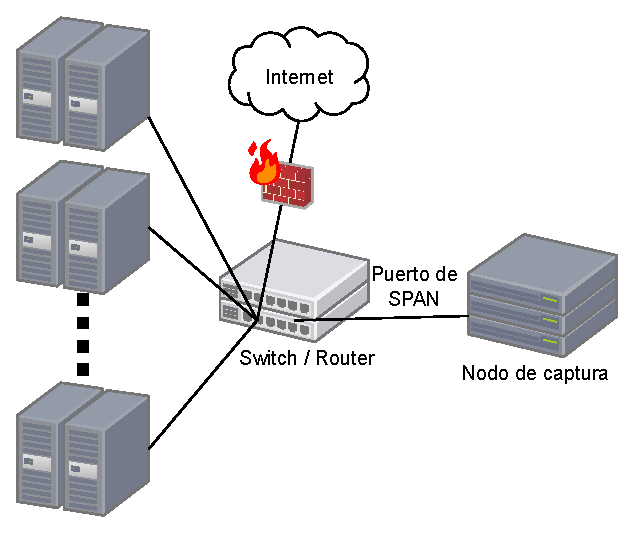
\includegraphics[scale=.7]{arq}
\caption{Arquitectura de captura tradicional}
\label{fig:dis:arq}
\end{figure}

No obstante, añadir un nuevo equipo a una red, suele suponer la implantación de un equipo grande (4\gls{u}) y de elevado coste dentro del \gls{cpd} en donde se encuentran los equipos y la red que desean ser monitorizados. También hay que tener en cuenta, que añadir un nuevo equipo supone una serie de riesgos de seguridad para la empresa propietaria de la red y de los equipos y que en ciertos casos, puede no ser asumible.

Dejando estos problemas de lado, es importante tener en cuenta que esta visión de como funciona un~\gls{cpd} y por ende, esta definición de la arquitectura de red es muy diferente a la visión tradicional. Actualmente, y desde la popularización del \gls{cloud}, resulta difícil de imaginar un dispositivo dedicado en exclusiva a una única tarea. De forma habitual, una aplicación (como puede ser un servidor web o una base de datos) no explota completamente los recursos de la máquina en la que se ejecuta. Por este motivo, los \glspl{cpd} actuales(Ver Fig.~\ref{fig:dis:arqvm}) disponen de grandes y potentes máquinas que permiten ejecutar multitud de pequeñas máquinas virtuales dedicadas a tareas muy concretas. Esta división en pequeñas tareas o servicios viene de la mano con el auge de los sistemas distribuidos (como Hadoop~\cite{hadoop,hadoop-definitive-guide}), cuyo objetivo es la resolución de un gran problema a base de fragmentarlo en pequeños trozos y procesarlos en paralelo.

%Arquitectura en un sistema virtual

\begin{figure}[!th]
\centering
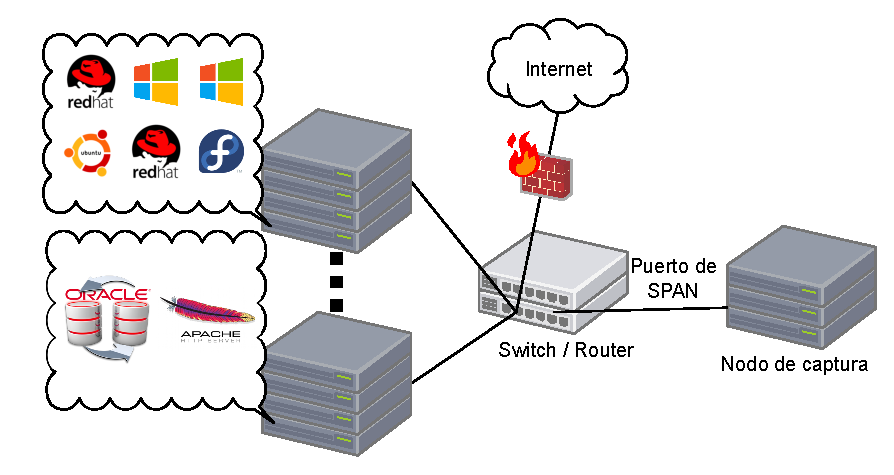
\includegraphics[scale=.7]{arqvm}
\caption{Arquitectura de captura en un sistema con virtualización}
\label{fig:dis:arqvm}
\end{figure}

La aparición de la virtualización, al igual que aumenta la rentabilidad de los servidores, hace surgir nuevos problemas que en un escenario tradicional no se presentaban. Dentro de un único servidor, están presentes varios sistemas operativos, así como sus respectivas aplicaciones. Comunicar las diferentes máquinas virtuales con el exterior supone una decisión crítica a la hora de definir cada una de las \gls{vm}.
Virtualizar las tarjetas de red con \textit{Passthrough} permite explotar las tarjetas de red al máximo, por otro lado, esto requeriría una tarjeta de red completa por cada una de las máquinas virtuales que fuesen a ejecutarse en la máquina física, además de un aumento en el número de cables y en la capacidad de los switches para interconectarlas.

Dada que una de las bases de las máquinas virtuales es la compartición de recursos, estas máquinas virtuales suelen utilizar virtualizaciones completas de las tarjetas de red, para virtualizaciones de las mismas, o en su defecto, \glspl{nfv}. Esta compartición de las interfaces de red, provoca que la tarjeta de red actué como un switch virtual entre las diferentes \glspl{vm} que la comparten. Aunque esto, a priori, no parece suponer un problema, hay que tener en cuenta que el objetivo es monitorizar el tráfico de una determinada red. Todo el tráfico interno entre máquinas virtuales no llega nunca a salir al nodo de captura de la figura~\ref{fig:dis:arqvm}, perdiéndose información potencialmente relevante para la motorización de la red.

%Arquitectura en un sistema completo virtual

\begin{figure}[!th]
\centering
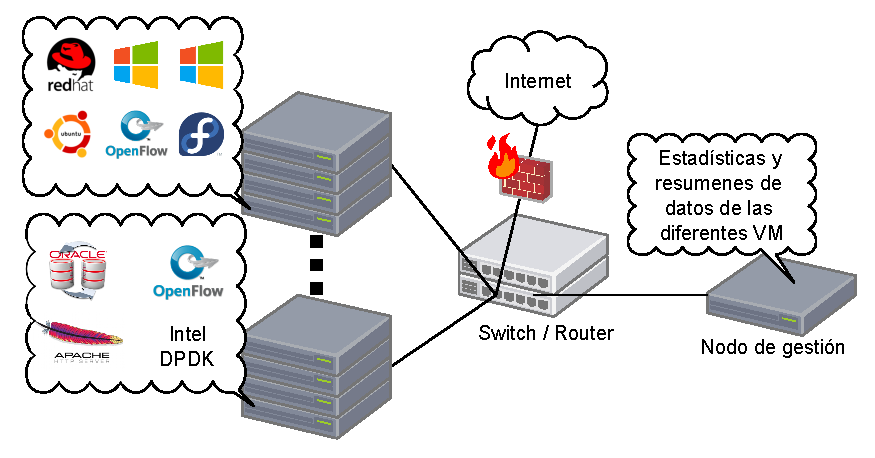
\includegraphics[scale=.7]{arqfullvm}
\caption{Arquitectura de un sistema de captura completamente virtualizado}
\label{fig:dis:arqfullvm}
\end{figure}

La única forma de solventar este problema, supone la inserción de un elemento en las máquinas anfitrionas que monitorice dicho tráfico. La forma mas simple de hacerlo, radica en insertar una máquina virtual en cada máquina física, de forma que recoja y procese el tráfico del resto de \glspl{vm} de su anfitriona.
En caso de lograr posicionar una \gls{vm} en cada nodo físico a monitorizar, la necesidad de disponer de una máquina de captura desaparece completamente. No obstante, al tener un conjunto de \glspl{vm} monitorizando fragmentos de la red, aparece el concepto de agente (o nodo) de gestión de monitorización. Este nodo, que bien puede ser un elemento físico u otra \gls{vm}, se encargaría de recoger la información capturada y procesada en las distintas \glspl{vm} de monitorización y centralizar los resultados bajo un único punto de acceso. La figura~\ref{fig:dis:arqfullvm} muestra una representación gráfica del escenario previamente descrito. Aunque está presente el elemento \textit{OpenFlow} en el dibujo, podría ser sustituido por cualquier otro agente de monitorización y captura de tráfico.

\lsection{Sistema de captura diseñado}

A raíz de los escenarios descritos previamente, es posible definir los requisitos que requiere nuestra aplicación de captura de red.
En el peor de los casos, esta aplicación debe ser capaz de capturar y almacenar el tráfico a tasa de linea, es decir: 10~\gls{gbps}.
Del mismo modo, la aplicación debe ser capaz de trabajar tanto en entornos físicos como en entornos virtuales (Ya sea mediante dispositivos \gls{virtio}, como \glspl{nfv}).
Para lograrlo, dicha herramienta, debe utilizar la API de Intel~\gls{dpdk} que implementa esta compatibilidad con elementos virtuales. \gls{dpdk} también ofrece una cierta interoperatividad con diferentes tarjetas de red, no limitando la aplicación a un único fabricante.

%El funcionamiento interno de esta API es muy conocido y ha sido estudiado previamente en trabajos anteriores~\cite{rleira2013TFG,dpdk:Leir1306}.

Para crear una aplicación con Intel~\gls{dpdk}, hay que tener en cuenta su filosofía orientada a la construcción de pipelines y explotación de paralelismo. El funcionamiento de comunicación entre diferentes elementos en una aplicación \gls{dpdk} se basa en la utilización de anillos. Cada anillo, está diseñado como una cola circular que almacena punteros a descriptores de paquetes. Cada descriptor de paquete, a su vez almacena el tamaño del paquete y un puntero al contenido del mismo. De esta forma, al mover un paquete entre diferentes hilos, no es necesario copiar el contenido del paquete, optimizándose los accesos y escrituras de memoria.

Con el objetivo inicial en mente, de evaluar \gls{dpdk} en el mejor caso posible (sin procesamiento), se ha desarrollado una aplicación con único hilo. Dicha aplicación captura todos y cada uno de los paquetes y libera los recursos asociados tan pronto es posible. Tras haber recibido un determinado número de paquetes, imprime por pantalla uno valor estimado de ancho de banda, así como cantidad de paquetes recibidos y perdidos (ya sea por errores en los paquetes u otros efectos). Dado que el funcionamiento en detalle de la API es muy conocido~\cite{dpdk2015} y ha sido estudiado previamente en trabajos anteriores~\cite{rleira2013TFG,dpdk:Leir1306}, considero que no es necesario entrar en detalles implementativos de la aplicación. En la figura~\ref{fig:dis:dpdktest} se muestra una representación gráfica del flujo de datos en la aplicación, mientras que en~\cite{dpdkspeedometer} puede descargarse la aplicación desarrollada.

\begin{figure}[!th]
\centering
\includegraphics[scale=.7]{dpdktest}
\caption{Arquitectura de un sistema de captura con DPDK}
\label{fig:dis:dpdktest}
\end{figure}

Una vez se ha desarrollado una versión preliminar capaz de capturar todos los paquetes a alta velocidad, es posible ampliar la aplicación y almacenar a disco. Aunque parezca una tarea sencilla, existe una serie de restricciones que deben tenerse presentes si se desea escribir a alta velocidad. Dichas restricciones vienen impuestas directamente por la tecnología de almacenamiento utilizada, que en este caso son discos duros.

Fundamentalmente pueden encontrarse 2 tipos de discos duros: Discos duros mecánicos y \glspl{ssd}. Cada tipo, tiene sus propias ventajas e inconvenientes. La unidad básica de escritura y lectura de un disco duro es el \textit{bloque} (típicamente con tamaños del ordern de KiloBytes o pocos MegaBytes). Si una aplicación desea leer o escribir un único byte en un disco duro, independientemente del sistema de ficheros que se esté utilizando, el sistema operativo deberá leer y/o escribir el bloque completo.
Los discos duros mecánicos se basan utilizan un conjunto de discos magnéticos para almacenar los datos. Dichos discos, deben girar a alta velocidad para ofrecer una velocidad de lectura razonable, así como un conjunto de agujas que se desplacen por el disco leyendo y escribiendo los diferentes bloques. Dichos bloques, se encuentran consecutivos, de forma que leer o escribir una gran cantidad de datos de forma consecutiva, suponga un movimiento muy sutil de las agujas y por tanto un rendimiento muy bueno. Por otro lado, leer o escribir en bloques disjuntos puede obligar a la aguja a moverse llegando a perderse del orden de milisegundos en el proceso.

En cambio, los discos duros \gls{ssd}, en cambio, utilizan memoria flash para almacenar los datos. Esta memoria, no tiene problemas de localidad, por lo que acceder a bloques muy esparcidos no supone una degradación del rendimiento. Esta tecnología, tambien ofrece unas mayores tasas tanto de lectura y escritura (unos 500~MBps, comparados con unos 150~MBps de los discos duros mecánicos). A cambio de estas ventajas, cada bloque de almacenamiento de un \gls{ssd} tiene limitados el número de escrituras posibles. De cara a realizar escrituras de forma periódica y dado el coste que supone un disco \gls{ssd}, parece más sensato utilizar discos duros mecánicos como método de almacenamiento.

No obstante, dado que el objetivo es capturar a 10~\gls{gbps}, es necesario utilizar un conjunto de discos. Gracias a las pruebas que se comentan en la sección~\ref{sec:equipamiento}, se ha determinado que gracias a un \gls{raid0} formado por 9 discos, es posible escribir a 10~\gls{gbps}. No obstante, alcanzar estas velocidades sigue sin ser una tarea del todo trivial. Al crear un \gls{raid0}, el tamaño de bloque del disco RAID se convierte en el tamaño de bloque de la suma de tamaños de bloque de cada uno de los discos que lo forman. Realizar escrituras más pequeñas que este tamaño, degradaría el rendimiento de escritura, por lo que hay que tenerlo presente.

Los sistemas operativos actuales, realizan una división entre la memoria que pertenece al usuario y la memoria que pertenece al núcleo ( o Kernel ) del sistema operativo. A la hora de realizar multitud de tareas, esta división acarrea problemas de rendimiento y el acceso a disco no es una excepción. Al solicitar una escritura de forma habitual en una aplicación de usuario, la información solicitada es copiada a una región específica del Kernel, y es desde esa memoria desde donde se transferirá al RAID. A la hora de trabajar a altas velocidades, esta copia intermedia impide alcanzar la tasa deseada. No obstante, es posible abrir un fichero en modo ``Direct'', es decir, que los datos sean copiados directamente desde la región de memoria del usuario, hasta el fichero destino. Tunear y refinar esta escritura en disco desde una aplicación propia lleva tiempo y en caso de tratarse de un \gls{raid0}, depende del número y propiedades de los discos que lo conforman.
Recordemos, que la herramienta debe producir un fichero estándar de los paquetes que ha capturado. El formato estándar para este cometido se denomina PCAP. Un fichero PCAP clásico está compuesto por una pequeña cabecera inicial, y una sucesión de estructuras paquete. Cada una de estas estructuras está formado a su vez por una cabecera en la que figura el tamaño del paquete, el tamaño capturado del paquete, el momento en el que se capturó el paquete y finalmente, el contenido capturado del propio paquete. Debido a que la mayoría de herramientas que procesan ficheros en este formato trabajan adecuadamente con ficheros grandes, la herramienta de captura debe trocear y generar una sucesión de ficheros de tamaño más o menos constante. De forma ideal, este tamaño debe ser de unos 2~GBs como máximo.

\newpage
Con todas estas ideas en mente, y partiendo del programa inicial presentado en la figura~\ref{fig:dis:dpdktest}, es posible describir la arquitectura final de la herramienta, la cual está formada por 3 hilos:

\begin{itemize}
\item \textbf{Hilo de captura}: Al igual que en la primera versión, un primer hilo se encarga de recoger los paquetes desde el anillo de recepción de la \gls{nic} de captura, sin realizar ningún cálculo con ellos, los inserta a alta velocidad en un nuevo anillo software.

\item \textbf{Hilo de construcción PCAP}: El segundo hilo es el encargado de realizar la mayor parte del procesamiento de paquetes. El trabajo de este hilo, consiste en la construcción de ficheros PCAP en memoria. Para lograrlo, cuenta con un array de buffers de 1~GB (por defecto de tamaño 4), en donde se almacenará en formato binario el fichero PCAP completo. Dado que el tamaño de un fichero puede ser superior al de un buffer, este hilo debe indicar que buffers representan un nuevo fichero y cuales representan la continuación del buffer predecesor. Por cada buffer de comienzo de fichero, el hilo escribe una cabecera de formato PCAP. A continuación comienza a extraer bloques de paquetes del anillo software mencionado anteriormente. Cada uno de estos paquetes, es marcado temporalmente mediante una \gls{hptl}~\cite{bib:hptl}, de forma que pueda construirse la cabecera del paquete. Tanto la cabecera, como el contenido del paquete son copiados al buffer.
Cuando el último paquete del último buffer que forma un fichero debe ser escrito, puede dejar algunos bytes libres en los que no quepa dl posible siguiente paquete. En estos casos, el hilo anota en el buffer, que el fichero debe ser truncado tantos bytes como hayan quedado en desuso. Una vez se ha completado el buffer, el hilo lo libera y comienza a trabajar con el siguiente buffer disponible.

\item \textbf{Hilo de volcado a disco}: El tercer hilo, es el encargado de volcar el contenido de los buffers intermedios a disco. Dado que el proceso de escritura es bloqueante, es necesario disponer de un hilo encargado únicamente a este proceso.
Gracias al funcionamiento de \gls{dpdk}, los buffers en los que escribe el segundo hilo se encuentran contiguos y alineados en memoria, de forma que el Kernel es capaz de escribirlo en el fichero destino a muy bajo coste. Este hilo, a su vez, es el encargado de la creación y truncado de ficheros, mediante las pautas indicadas por el hilo número 2. Tras terminar el volcado de un buffer, el hilo lo libera para que pueda ser reutilizado cuanto antes. 
\end{itemize}

Gráficamente, es posible ver la arquitectura y el flujo de los paquetes en la figura~\ref{fig:dis:dpdkdd}.

\begin{figure}[!th]
\centering
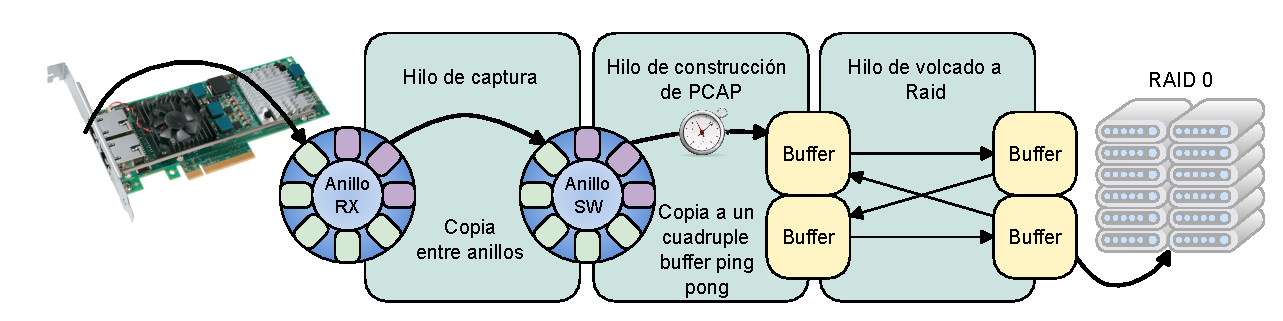
\includegraphics[scale=.7]{dpdkdd}
\caption{Arquitectura de un sistema de captura y almacenamiento con DPDK}
\label{fig:dis:dpdkdd}
\end{figure}













%
% Desarrollo
%
\chapter{Pruebas\label{sec:desarrollo}}

El objetivo de este capítulo es mostrar tanto las pruebas realizadas como la metodología seguida para obtener los resultados.
Para poder entrar en detalle, en las pruebas, es necesario hacer un repaso de los dispositivos hardware y software que se encuentran disponibles. Una vez conocidos, es posible definir una metodología de pruebas, así como una descripción de las mismas en los diferentes entornos.

\lsection{Entorno de Desarrollo\label{sec:entorno}}

Escoger un entorno de desarrollo y pruebas adecuado, supone realizar multitud de comparativas y pruebas entre los diferentes elementos disponibles, tanto a nivel software, como a nivel hardware.
Poner a prueba todos y cada uno de los posibles elementos supone un reto en cuanto a coste monetario como en tiempo, y dado que tanto el presupuesto como el tiempo de realización del doble trabajo fin de máster son finitos, se ha partido del siguiente equipamiento facilitado por el grupo de investigación HPCN.

\subsection{Equipamiento de prueba utilizado\label{sec:equipamiento}}

El equipamiento de prueba utilizado costa de 3 elementos fundamentales: Captura de tráfico, emisión de tráfico y el tráfico emitido como tal.
Todos estos elementos son de vital importancia a la hora de realizar una comparativa, pues tan importante es el proceso de captura, como que los datos recibidos hayan sido emitidos correctamente. Estos datos, por otro lado, deben representar algún tráfico significativo para las pruebas, ya sea un caso extremo, o un caso realista. Cada una de estas partes es explicada con detalle a continuación:
\\
\\

\subsubsection{Equipo de captura y desarrollo}

El equipo de captura y desarrollo es conocido internamente por el nombre de \textit{Nrg}.
Esta sonda de captura, está compuesta por una arquitectura de tipo \gls{numa} con dos procesadores \textit{Intel Xeon E5-2630} a una velocidad de 2.6~Ghz cada uno.
Ambos procesadores se encuentran conectados a 2 tarjetas de memoria de 8~GB cada una, haciendo un total de 32~GB para todo el sistema.
Este equipo cuenta con diversos PCIe generación 3 que permiten transferencias de datos de hasta casi un 1~\gls{gbps} por cada linea PCIe. El equipo cuenta con los siguientes dispositivos PCI:

\begin{itemize}
\item \textbf{Tarjeta gráfica Nvidia Tesla K40C}: A pesar de no haber sido utilizada la tarjeta gráfica a lo largo de las pruebas o el desarrollo, parece interesante mencionar su presencia en el bus PCIe.

\item \textbf{Tarjeta de red Ethernet Mellanox MT27500 (ConnectX-3)}: Esta tarjeta es capaz de establecer velocidades de enlace de entre 40 y 56~\gls{gbps}. Aunque inicialmente se pretendía probar esta tarjeta, Intel~\gls{dpdk} no publicó los drivers para explotar esta tarjeta hasta la versión 2.0, la cual fue publicada en abril de 2015. De igual modo, no disponemos de ningún emisor de tráfico fiable capaz de saturar este enlace, ni tampoco la capacidad de realizar el almacenamiento a disco a esta tasa de red sin realizar algún tipo de filtrado de tráfico. Hasta donde llega mi conocimiento, no existe (aparte del nuevo driver de Intel~\gls{dpdk} y el driver nativo) ninguna aplicación similar contra la que comparar resultados. Por todo esto, el uso de esta tarjeta ha sido descartado al encontrarse fuera del marco de este trabajo. Esta tarjeta conecta la máquina de captura con la máquina llamada \textit{Onelab3}.

\item \textbf{Tarjeta de red Ethernet Intel I350}: Esta tarjeta dispone de dos \glspl{nic} a 1~\gls{gbps} cada una. Dado la máquina de captura se encuentra inaccesible físicamente, se ha utilizado esta tarjeta como medio para el acceso remoto, así como el acceso a diferentes recursos y paquetes de Internet.

\item \textbf{Tarjeta de red Ethernet Intel 82599ES}: Esta tarjeta dispone de dos \glspl{nic} SFP+ a 10~\gls{gbps} cada una. El chipset \textit{82599ES} es compatible con la mayoría de capturadores de bajo coste actuales, por lo que la convierte en el dispositivo predilecto de cara a realizar una comparativa de rendimiento. Además, soporta diferentes modos de virtualización (\gls{passthough} y \gls{sriov}), permitiendo de esta forma alcanzar los objetivos planteados en este trabajo. Las dos interfaces de la tarjeta se encuentran conectadas al emisor de tráfico (llamado \textit{Dagda}), el cual será explicado más adelante.

\item \textbf{Controladora MegaRAID SAS-3 3108}: Dadas las limitaciones del chasis de la sonda de captura, la controladora RAID es capaz de gestionar hasta un máximo de 12 discos duros. Estos discos duros, pueden conformar desde un único Raid 0, hasta un conjunto de diferentes tipos de Raid. 
\end{itemize}

%seria interesante preguntar a victor por paper de referencia
Una vez observados los diferentes dispositivos disponibles, parece interesante realizar un inciso en la controladora raid.
Si bien puede gestionar hasta 12 discos duros, el precio de estos no es en absoluto despreciable.
En este caso, se parte de discos mecánicos \textit{Hitachi HUA 72303} (especiales para servidores) con 3~TB de capacidad cada uno.
El precio actual aproximado de estos discos duros oscila entorno a los \textit{310€}, elevando el coste de almacenamiento a más de \textit{3700€}.
Por este motivo, determinar cual es la cantidad de discos duros necesarios para cada escenario es de vital importancia de cara a reducir el coste de la sonda de captura.


\subsubsection{Equipo de emisión de tráfico}

Existen multitud de herramientas de emisión de tráfico.
Una de las herramientas clásicas es \href{http://tcpreplay.appneta.com/}{TCPReplay}.
Dicha herramienta parte de un fichero estándar \textit{PCAP} y lo transmite por una determinada interfaz de red. TCPReplay, proporciona cierto valor añadido, ya que puede regular la velocidad de transmisión entre otras muchas cosas. No obstante, esta herramienta al igual que la mayoría de emisores de tráfico clásicos (Como pktgen, etc), no es capaz de emitir tráfico a 10~\gls{gbps}, aun si este se encuentra en memoria. Esto se debe a que las herramientas de transmisión y generación de tráfico utilizan la pila de red completa del Kernel y los drivers \gls{vanilla} de las tarjetas de red.

De cara a solventar el problema de la generación y transmisión de tráfico, se han construido multitud de herramientas. Los generadores de tráfico software se basan en la reutilización de los drivers optimizados de captura como \gls{dpdk} o \textit{PacketShader}. No obstante, los emisores de tráfico software presentan serias limitaciones.
%
En el caso del emisor de \textit{PacketShader}~\cite{dpdk:packetshader}, se presentan ciertas irregularidades en la tasa de tráfico: emisión a ráfagas, problemas en los contenidos de los paquetes y en general problemas de estabilidad. De cara a hacer una comparativa de rendimiento y tasa de captura, estas irregularidades complicarían y harían fluctuar las medidas, por lo que este emisor fue descartado.
%
Por otro lado, Intel \gls{dpdk} proporciona una herramienta de emisión de tráfico bastante sofísticada conocida como \textit{Pktgen-\gls{dpdk}}~\cite{bib:dpdkpktgen}, la cual, poco a poco, se está convirtiendo en una conocida aplicación. 
La herramienta \textit{Pktgen} es capaz de saturar fácilmente 4 enlaces a 10~\gls{gbps} mediante tráfico sintético. Para conseguirlo, reserva las estructuras de los paquetes en memoria y las envía a cada una de las \gls{nic}. Esta herramienta, aunque útil para probar casos extremos, se ve perjudicada si lo que se desea es enviar tráfico almacenado previamente en un fichero. Debido al sobrecoste de las estructuras de los paquetes%
\footnote{Cada estructura de \gls{dpdk} almacena diversa información referente a un paquete. De cara a mantener la coalescencia de las cachés, estas estructuras cuentan con 2048 Bytes (La potencia de 2 más próxima a la \gls{mtu} de la red) para almacenar el payload del paquete.}%
 que utiliza \gls{dpdk}, no es posible almacenar más que unos pocos centenares de miles de paquetes por GigaByte. Aunque este número pueda aparentar ser muy grande, recordemos que en una red de 10~\gls{gbps}, se pueden llegar a mandar hasta casi 15 millones de paquetes por segundo (en caso de paquete mínimo), por lo que esta cantidad de paquetes representaría menos de una décima parte de segundo del tráfico del enlace.
 
En el otro lado, se encuentran los generadores hardware basados en \glspl{fpga}. Dentro del grupo de investigación HPCN ha sido desarrollado un potente y versátil generador de tráfico a 10~\gls{gbps}~\cite{zazo2014tnt10g}. Este generador, aporta un nivel de control en la transmisión de las tramas muy preciso, permitiendo simular, tanto cualquier situación de una red real, como casos extremos incluso a nivel físico.
Para lograr estas características, este sistema utiliza un formato especial de fichero denominado \textit{simple}. Este fichero es similar al formato PCAP, salvo porque almacena la cantidad de ceros que existen a nivel físico entre dos paquetes, lo que permite tener un elevado control y precisión durante la emisión. Dichos ficheros se encuentran en un Raid 0, de forma que un driver intermedio es capaz de acceder de forma eficiente a ellos y copiarlos en \glspl{huge}. Estas páginas son transferidas a la \gls{fpga} a través del bus PCIe. La \gls{fpga} emite el tráfico por una o varias de las diferentes \gls{nic} que posee. Como contrapartida, aunque la \gls{fpga} dispone de hasta 4 interfaces de 10~\gls{gbps}, solo es capaz de recibir hasta 10~\gls{gbps} por PCIe, por lo que como mucho podrá enviar el mismo tráfico simultáneamente por las diferentes \glspl{nic}. En la figura~\ref{fig:rafaDagda} se muestra un esquema del funcionamiento del generador y emisor de tráfico hardware.

\begin{figure}[!htb]
\centering
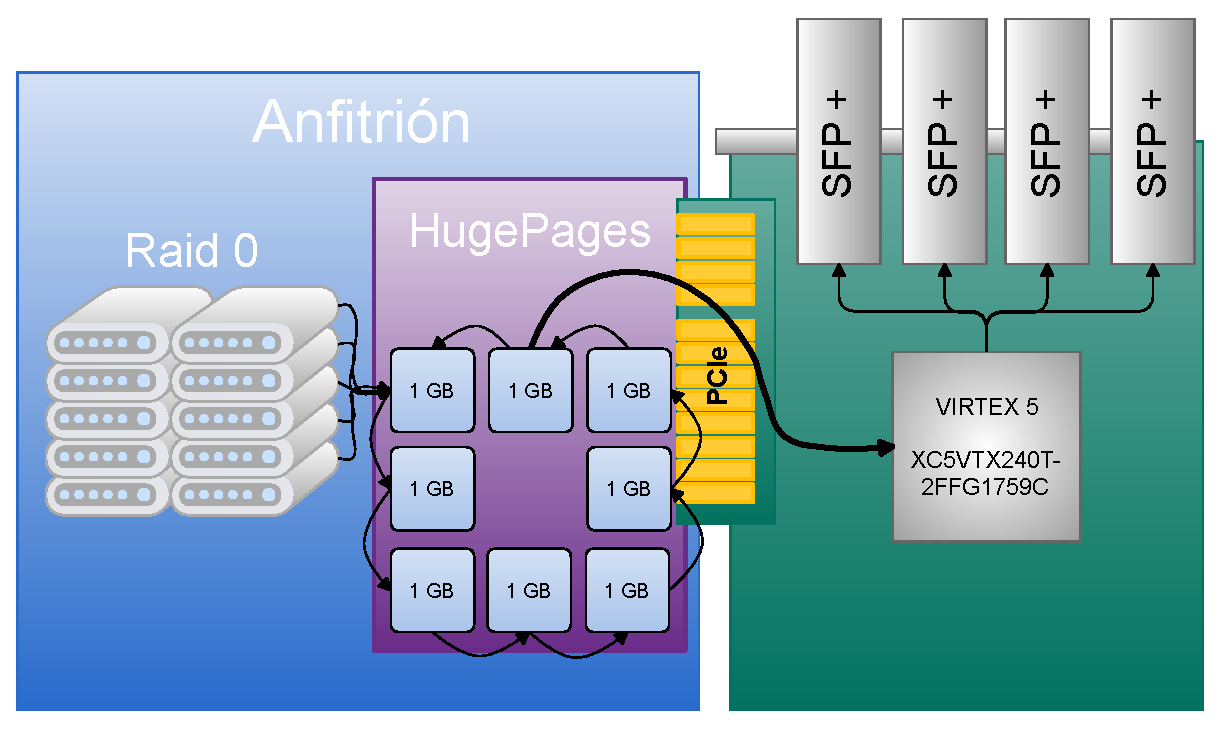
\includegraphics[scale=.6]{rafaDagda}
\caption{Arquitectura del emisor de tráfico}
\label{fig:rafaDagda}
\end{figure}

Tras escoger el generador de tráfico hardware, se definió un interconexionado de las diferentes máquinas que formarán parte de las diversas pruebas. La máquina encargada de la transmisión de tráfico (llamada \textit{Dagda}) se conecta mediante 2 interfaces de 10~\gls{gbps} a la máquina capturadora de tráfico (llamada \textit{Nrg}). La máquina de captura se encuentra a su vez conectada por un enlace de 40~\gls{gbps} con una máquina llamda \textit{Onelab3}. No obstante, y como se ha mencionado anteriormente, este enlace queda en desuso debido a la falta de software necesario para explotarlo adecuadamente. En la figura~\ref{fig:conexiones} se muestra gráficamente este interconexionado.

\begin{figure}[!htb]
\centering
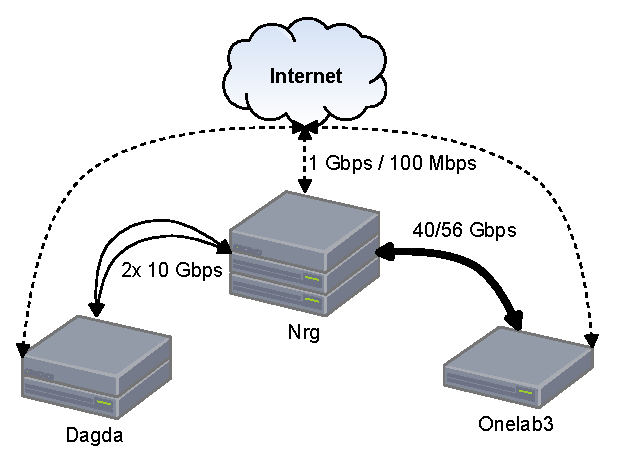
\includegraphics[scale=.8]{conexiones}
\caption{Conexionado del equipo de captura y desarrollo}
\label{fig:conexiones}
\end{figure}

\subsubsection{Tráfico emitido}

Una vez se ha decidido tanto el funcionamiento de la sonda de captura, como el hardware que se utilizará, es necesario definir el tráfico con el que se realizarán las evaluaciones, pruebas y comparativas. Para poder tener medidas útiles, es necesario poner al equipo de captura al límite, forzando y poniendo el sistema en el peor caso posible. No obstante, como se comentó en la introducción, resulta complicado encontrar enlaces completamente saturados, por lo que resulta interesante contar con tráfico representativo real.

Con el objetivo de cubrir ambos escenarios, se han utilizado los siguientes tipos de tráfico:

\begin{enumerate}

\item \textbf{Tráfico extremo}: Dentro del protocolo Ethernet, existen dos casos peores posibles: Un enlace en la que solo hay paquetes de 64 bytes y supone una tasa de 14.88 Millones de paquetes por segundo, o un enlace, en la que solo hay paquetes de tamaño 1500 y unos 800 mil paquetes por segundo.
En el primer caso, tan solo un 76\% de los bytes transmitidos%
\footnote{Los paquetes Ethernet tienen diversos campos, como el interframe gap o el preludio, que deben ser transmitidos pero no aportan ninguna información relevante. Por este motivo, dichos campos nunca son transmitidos por la tarjeta hacia el ordenador anfitrión y no pueden ser almacenados. En caso de que los paquetes sean muy pequeños, estos bytes ``ocultos'' se hacen relevantes.} %
 en el enlace son almacenados, mientras que en el segundo caso se almacenan entorno al 98\% de los bytes. Mientras que el primer caso requiere una mayor necesidad de computo para procesar un gigantesco número de paquetes, el segundo caso requiere de una mayor capacidad de escritura a disco.
Las herramientas proporcionadas por el generador de tráfico hardware escogido, son capaces de generar ambos escenarios extremos sin la necesidad de construir una traza a medida para la prueba.

\item \textbf{Tráfico Real}: Para poder obtener a tráfico real representativo a alta velocidad, es necesario recurrir a redes de grandes empresas o grandes nodos de interconexión de algún \gls{isp}. Esto causa, que la naturaleza de este tipo de tráfico suela ser confidencial o deba mantener ciertos requisitos de privacidad, por lo que, es complejo acceder a este tipo de muestras de tráfico.
Dentro de este contexto, la organización \href{http://www.caida.org/home/}{Caida}, captura tráfico en nodos que interconectan grandes ciudades de Estados Unidos. Tras realizar un proceso de anonimización\footnote{El proceso de anonimización consiste en truncar los paquetes eliminando la capa de aplicación.}, la organización Caida publica estas capturas de tráfico para su posterior uso por investigadores. Dentro de las trazas disponibles, se ha escogido una muestra unos 7 minutos de duración entre la ciudad de Seattle y la ciudad de Chicago el día 1 de octubre de 2014~\cite{caida2014}. Aunque esta traza está capturada en un enlace a 10~\gls{gbps}, la velocidad efectiva del tráfico ronda los 5~\gls{gbps} con un tamaño medio de paquete de unos 965 Bytes. De cara a realizar las pruebas y estresar un poco el sistema, se ha decidido acelerar transmisión de esta traza, reduciendo el tiempo entre los paquetes al mínimo posible.

\end{enumerate}

\subsection{Software utilizado\label{sec:sw}}

Encontrar el software apropiado para realizar un desarrollo es una tarea tediosa. Dado que el objetivo de este trabajo fin de máster es la realización de un motor de captura y almacenamiento de tráfico con Intel~\gls{dpdk} y la realización de una comparativa entre los diferentes métodos de captura en diferentes entornos de ejecución, es necesario plantear un entorno software aceptable para un posible cliente.
%
En el mundo empresarial, predomina el uso de las distribuciones de linux basadas en red hat o en suse. No obstante, la tecnología de virtualización, requiere de los últimos avances para poder ser explotada al máximo. Con esto en mente, la distribución de linux que mejor cumple estas condiciones es Fedora. Por este motivo, en la sonde captura se ha instalado un Fedora 20.

La mayoría de los entornos de virtualización de los que disponen las grandes compañías son: \gls{kvm}~\cite{bib:kvm}, XEN~\cite{bib:xen} o la versión profesional de VMWare~\cite{bib:vmware}. De cara a un presupuesto limitado, descartamos la opción de utilizar VMWare desde el principio. La decisión entre los hypervisores \gls{kvm} y XEN es algo más compleja pues son ambos sistemas muy utilizados, ambos son gratuitos y ambos se encuentran en auge. No obstante, se aprecia a la comunidad investigadora más enfocada en el entorno de \gls{kvm}, así como una gran cantidad de esfuerzo por parte de la comunidad de \gls{kvm} en el desarrollo de elementos y técnicas avanzadas de virtualización como \gls{virtio}. Por estos motivos, se ha escogido \gls{kvm} como método de virtualización.
%
Como optimización, dado que varios de los motores de captura hacen uso de las \glspl{huge}, se ha configurado el sistema de virtualización \gls{kvm} para que reserve la memoria de las máquinas virtuales en \gls{huge} con el objetivo de que el rendimiento en las \glspl{vm} no se vea excesivamente afectado por problemas de paginación o problemas de cache~\cite{kudryastev2013pcs}. Las máquinas virtuales, a su vez, proveen \gls{huge} a los diferentes motores que se ejecutan en ellas.
%
Cada una de las máquinas virtuales utilizadas está formada por 3 \glspl{core} virtuales, mapeados y reservados en 3 \glspl{core} físicos. Cada máquina virtual cuenta a su vez con 5~GB de memoria RAM.

Una vez que tenemos los más pilares básicos de nuestro sistema de captura, es necesario hacer un pequeño énfasis en lo que a funciones virtuales se refiere. Tal y como se ha explicado en capítulos anteriores, las funciones virtuales son a todos los efectos un dispositivo PCIe más. No obstante, las tarjetas Intel ofrecen diversas formas de crear y gestionar sus \glspl{nfv}. Por un lado, el driver \gls{vanilla} \textit{ixgbe}, permite indicar a la tarjeta que cree un número determinado de \glspl{nfv}, de una forma muy sencilla. No obstante, este tipo de funcionamiento delega todo el control de la función virtual a la tarjeta física, sin que la CPU intervenga en ningún caso en el trasiego de paquetes.
%
Por otro lado, el driver proporcionado por \gls{dpdk}, proporciona su propia forma de gestionar las funciones virtuales. Este paradigma, rompe ligeramente el concepto de \gls{vf}, ya que \gls{dpdk} requiere del uso de un determinado programa, llamado \textit{testpmd}, que de forma activa ayuda a la tarjeta a manejar las diferentes funciones virtuales. No obstante, este método obliga a la \gls{cpu} a trabajar, consumiendo, como mínimo, un \gls{core} completo. De cara a evaluar que método es el mejor, se han tenido en cuenta ambas aproximaciones y se detallan los resultados de la comparativa en la sección~\ref{sec:sriov}.

Dentro del software de captura de tráfico se ha decidido realizar una comparativa entre los siguientes motores: \gls{dpdk}, \textit{HPCAP}, \textit{PF\_RING}, y el driver \gls{vanilla} \textit{ixgbe} mediante el programa de captura simple basado en \textit{libPCAP}~\cite{bib:tcpdump}.%\textit{TCPDump}~\cite{bib:tcpdump}. 
El resto de motores de captura han sido descartados para las pruebas, dado que su funcionamiento es muy similar entre sí, y ninguno de ellos es capaz de operar con~\gls{nfv}. Los motores de captura han sido explicados previamente en el capítulo~\ref{sec:estado_del_arte}.

\lsection{Metodología de las pruebas\label{sec:metod}}

Realizar todas y cada una de las pruebas que se describen en las siguientes secciones, supone un trabajo tedioso y en un principio muy manual. Si bien son importantes los resultados de las pruebas, es de igual importancia mantener un cierto protocolo a la hora de realizarlas asegurando su repetibilidad así como almacenar los resultados de forma organizada. 
Para llevar esto a cabo, se realizó un documento interno que incluían los pasos a la hora de lanzar una prueba en los diferentes escenarios, así como los parámetros recomendados para cada una de las diferentes aplicaciones.

Cada una de las aplicaciones de captura tiene su propia forma de representar las diferentes estadísticas relacionadas con la \gls{nic} que está utilizando para capturar (como paquetes recibidos, paquetes perdidos, paquetes con errores, etc).
De cara a normalizar estos datos, se realizaron diferentes scripts encargados de interpretar la salida de cada una de las aplicaciones y convertirlas a un formato único. El formato planteado se basa en un simple fichero de texto de 4 columnas separadas por tabulaciones. Cada línea de este fichero, representa un determinado instante de tiempo en el que se consultaron las estadísticas de una única \gls{nic}. En caso de que la aplicación esté gestionando más de una interfaz de red, se generan tantos ficheros como \glspl{nic} utilice.

El fichero de estadísticas de una \gls{nic} consta de las siguientes columnas:

\begin{enumerate}
\item Momento en formato unix en el que se realizó la medida.
\item Velocidad en Gigabits por segundo entre el momento anterior y el actual.
\item Paquetes recibidos entre el momento anterior y el actual.
\item Paquetes perdidos entre el momento anterior y el actual.
\end{enumerate}

Para poder mantener una organización entre las diferentes pruebas, estos ficheros son almacenados en un árbol de carpetas. Este árbol se subdivide en nombre de la prueba, tráfico utilizado, motor de captura utilizado y marca temporal del inicio de la prueba.
Dado que estos ficheros representan una serie temporal, que aporta cierta información de depuración, se ha realizado un nuevo script que resume los diferentes ficheros asociados a cada prueba, generándose así un pequeño informe de resultados de cada una de las pruebas realizadas.

La complejidad de los capturadores de tráfico es elevada. Por ello, estas aplicaciones cuentan con multitud de parámetros que los permiten acomodarse a diversos entornos. Estos parámetros engloban desde el \gls{core} en el que se ejecuta un determinado componente del capturador, hasta el tamaño de los descriptores de paquete o la longitud de las colas de recepción.
%
Para que la comparativa entre los diferentes motores de captura sea justa, es necesario repetir multitud de veces determinadas pruebas en busca de los parámetros adecuados. Del mismo modo, es necesario que todas las pruebas se ejecuten en las mismas condiciones, evitando fluctuaciones debido a otros efectos colaterales de haber ejecutado anteriormente una prueba con otro capturador (como elementos cacheados o cambios colaterales en el funcionamiento de algún dispositivo). Por este motivo, se desarrollaron dos protocolos de realización de pruebas, una para entornos físicos y virtuales mediante \gls{passthough} y otro para entornos virtuales con \glspl{nfv}:

\begin{itemize}
\item \textbf{Procedimiento en entorno físico y virtual con \gls{passthough}:}
\begin{enumerate}
\item Se reinicia la máquina (física o virtual) con la configuración adecuada (\glspl{huge} si son necesarias, etc).
\item Se resetea el generador de tráfico.
\item Se instancia el driver y programa de captura.
\item Se inicia la transmisión de tráfico por parte del generador.
\item Al terminar la ejecución del programa de transmisión, se cierra el programa de captura y se almacenan los resultados.
\end{enumerate}

\item \textbf{Procedimiento en entorno virtual con \gls{nfv}:}
\begin{enumerate}
\item Se instancia el driver encargado de la generación de \gls{nfv} y se configura.
\item Se reinicia la máquina virtual con la configuración adecuada a la prueba.
\item (Si procede) se inicia el programa \textit{testpmd} de Intel~\gls{dpdk} en el anfitrión.
\item Se resetea el generador de tráfico.
\item Se instancia el driver en la máquina virtual y programa de captura.
\item (Si procede) se configura el programa \textit{testpmd}.
\item Se inicia la transmisión de tráfico por parte del generador.
\item Al terminar la ejecución del programa de transmisión, se cierra el programa de captura y se almacenan las estadísticas tanto de la máquina virtual como de la máquina física.
\end{enumerate}

\end{itemize}

\lsection{Pruebas en entorno físico\label{sec:fisico}}

El régimen clásico de funcionamiento de las múltiples herramientas de red es el entorno nativo o físico. Dado que estas herramientas usualmente requieren de una gran cantidad de procesamiento así como de ancho de banda en la memoria para funcionar a altas (e incluso no tan altas) velocidades, hasta hace poco era impensable llevar a estas herramientas a un entorno virtual, salvo para realizar tareas con muy poca cantidad de datos.
Por este motivo, el entorno físico es el punto de partida en la realización de cualquier comparativa de herramientas de red, lo que incluye a los capturadores de red.

La arquitectura del entorno físico es simple. Una tarjeta de red y una controladora Raid, mediante sus correspondientes drivers, se conectan a un motor de captura. De esta forma, el trabajo del motor de captura se resume en una copia de los datos que llegan desde la red hasta el Raid de alta velocidad. En un principio, esta tarjeta de red, se encontraría conectada a un switch o a un router de la red que deseamos monitorizar, el cual, nos duplica todo el tráfico que circula por la misma mediante un puerto de SPAN. Dado que en este caso, no se ha podido acceder a una red de alta velocidad, se ha simulado este enlace mediante el generador hardware comentado previamente.

Si el servidor de captura es suficientemente potente, es posible que en paralelo se encuentren en ejecución otras aplicaciones en nuestra sonda de captura. Estas aplicaciones pueden encargarse de leer los datos almacenados en el Raid y sacar algún tipo de análisis, o incluso, ejecutar algún tipo de servicio que no esté directamente relacionado con la captura como un servidor web o una máquina virtual completa. Esta arquitectura puede verse en la figura~\ref{fig:vmfisica}.

\begin{figure}[!htb]
\centering
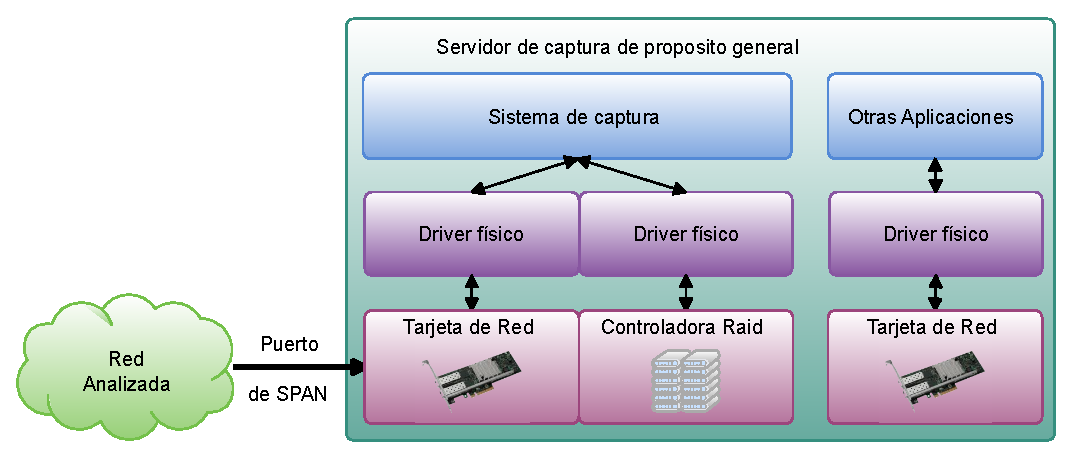
\includegraphics[scale=.6]{VMfisica}
\caption{Arquitectura de captura clásica}
\label{fig:vmfisica}
\end{figure}

Un sistema de captura y almacenado, como su nombre indica, se divide en dos partes: captura y almacenado. Ambos sistemas utilizan y explotan al máximo el ancho de banda de la memoria y el ancho de banda de los diferentes buses de comunicaciones. Por ello, es necesario realizar una comparativa que mida el caso mejor de ambos procesos por separado.

De cara a hacer una prueba de rendimiento del sistema de almacenado (Raid 0), se ha reutilizado un script que permite, dinámicamente, cambiar el número de discos que conforman el Raid de captura. Ya que los motores de captura de los que se dispone, almacenan sucesivos ficheros de 2~GB, este script se encarga también de realizar sucesivas escrituras de ficheros de 2~GB mediante la herramienta de \textit{GNU}, \textit{dd}. Tal y como se ha comentado anteriormente, para poder escribir a esta velocidad en un raid es necesario saltarse las copias intermedias que realiza de forma natural el kernel de \textit{Linux}. Para lograrlo, existe el modo de escritura \textit{Direct}, que permite al kernel copiar directamente desde la memoria del usuario a nuestro raid de captura.


\begin{figure}[!htb]
\centering
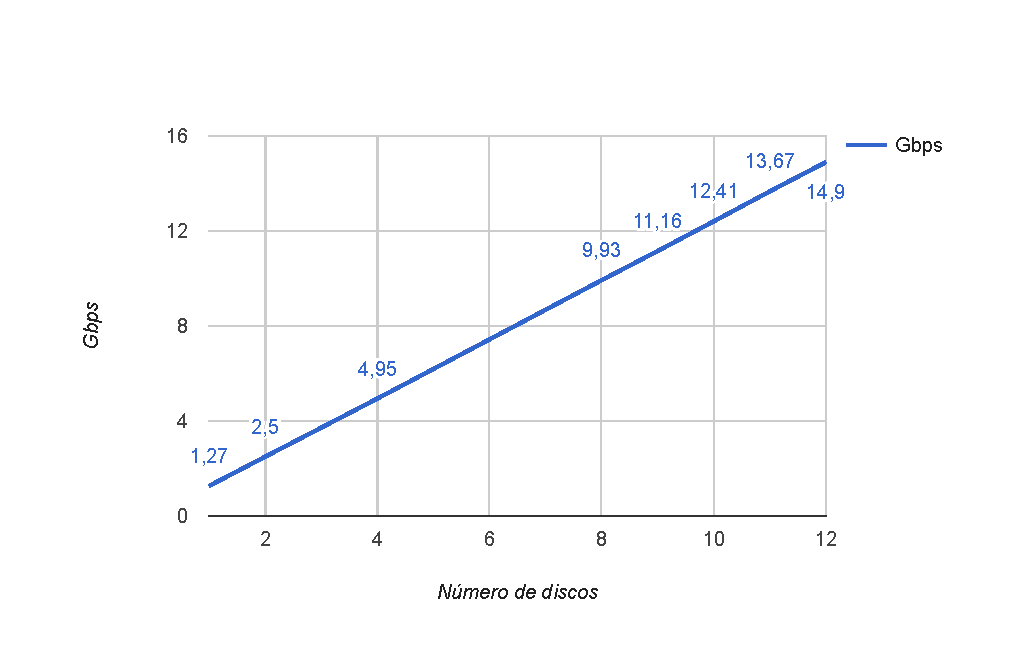
\includegraphics[scale=.7]{graph1}
\caption{Rendimiento de escritura en Raid 0 sin virtualización}
\label{fig:vmfisica:graphdd}
\end{figure}

Tal y como puede observarse en la figura~\ref{fig:vmfisica:graphdd}, la tasa de escritura a disco parece crecer de forma lineal con el número de discos que conforman el raid. A raíz de estos resultados, parece viable crear un raid de tan solo 9 discos para las pruebas, pues en media ofrece una tasa de escritura de más de los 10~\gls{gbps} a los que se recibe el tráfico. No obstante, y para mayor seguridad, se han realizado varios cientos de prueba de escritura para poder obtener un intervalo de confianza del rendimiento que proporciona el Raid con 9 discos. Dicho intervalo se encuentra entre 11,09 y 11,23~\gls{gbps}, lo que nos asegura en cierta medida que el rendimiento será suficiente para almacenar todo el tráfico.

Una vez se ha medido el rendimiento del raid de almacenamiento el caso óptimo, es posible comenzar a realizar las primeras pruebas de captura con los diferentes motores.
Dado que en esta primera prueba, se busca encontrar las limitaciones de los capturadores de tráfico, se han utilizado unas pequeñas aplicaciones que tan solo reciben el tráfico y no realizan ningún procesado sobre los mismos. Mientras que los motores \textit{HPCAP} y \textit{PF\_RING} proporcionan sus propias herramientas básicas de testeo, se ha realizado una herramienta propia en \gls{dpdk} para realizar este tipo de mediciones. De igual modo, se ha reutilizado una pequeña aplicación realizada en \textit{libpcap} para probar la tasa de captura del driver \gls{vanilla} \textit{ixgbe}.

Los resultados de esta primera prueba, pueden observarse en la tabla~\ref{tab:vmfisica:soloCap}. Estos resultados, resultan en cierta medida sorprendentes pues el driver \gls{vanilla} de Intel ha mejorado en gran medida con los años, pudiendo incluso capturar 10~\gls{gbps} sin perdidas cuando se enfrenta a un tráfico realista.
También cabe destacar, el rendimiento del motor de captura \textit{PF\_RING}. A pesar de obtener un buen rendimiento al enfrentarse a una única \gls{nic}, el rendimiento decrece y comienza perder paquetes cuando debe enfrentarse a 2 interfaces de red simultáneamente.
El rendimiento de \textit{HPCAP}, parece bastante razonable si recordamos su filosfía de \gls{onecopy}. Finalmente, en esta tabla se puede observar como la tecnología de captura más novedosa sale ganando en esta prueba sin llegar a perder ni un solo paquete en ninguna de los casos.

\begin{table}[htb]
\centering
\begin{tabular}{|c|c|c|c|c|}
	\hline
		\multirow{3}{*}{\begin{tabular}[c]{c}{\bf Motor}\\ {\bf de captura}\end{tabular}} & \multicolumn{4}{c|}{{\bf \% de paquetes procesados}}\\
	\cline{2-5}
		 & \multicolumn{2}{c|}{{\bf 1 \gls{nic}}} & \multicolumn{2}{c|}{{\bf 2 \glspl{nic}}} \\
	\cline{2-5}
		 & {\bf 64 Bytes }   & {\bf CAIDA}  & {\bf 64 Bytes}   & {\bf CAIDA}  \\ \hline
		ixgbe         & 2.7   & 100  & 3.7     & 93.55  \\ \hline
		PF\_RING      & 100   & 100  & 76.1    & 100    \\ \hline
		HPCAP         & 97.9  & 100 & 97.8  & 100     \\ \hline
		DPDK          & 100   & 100  & 100     & 100  \\ \hline
\end{tabular}
\caption{Porcentaje de paquetes capturados en un escenario sin virtualización ni almacenamiento de paquetes.}
\label{tab:vmfisica:soloCap}
\end{table}

Una vez se han obtenido los resultados de las primeras pruebas, es posible comenzar a realizar las pruebas conjuntas de captura y almacenamiento a disco. Cabe recordar, que en estas pruebas pueden empezar a surgir cuellos de botella en los accesos a memoria, así como en los accesos a los buses PCIe. Tal y como se muestra en la tabla~\ref{tab:vmfisica:CapAlmac}, el rendimiento con respecto a la tabla~\ref{tab:vmfisica:soloCap} decrece en cierta medida. Un detalle a tener en cuenta es el descenso en el rendimiento de la aplicación desarrollada en \gls{dpdk}. Al igual que el \gls{zerocopy} ayuda a mejorar el rendimiento, si el pipeline de proceso tiene demasiada latencia, se comienza a perder paquetes. Por otro lado, en una filosofía \gls{onecopy}, como la de \textit{HPCAP}, se independiza mucho mejor el procesamiento sobre los paquetes (en este caso copia a disco) del proceso de captura.
Por este motivo, la tasa de paquetes capturados utilizando \textit{HPCAP} se ve muy poco afectada cuando se añade el proceso de almacenado. Mientras que en la implementación de captura sobre \gls{dpdk}, se pierde más de un 4\% de los paquetes, frente a la implementación de solo captura que no perdía ningún paquete.
Finalmente, cabe mencionar que las pruebas sobre captura y almacenamiento se han realizado utilizando una única \gls{nic}. Dado que las pruebas del raid indican que solo es capaz de almacenar hasta 10~\gls{gbps}, carece de sentido realizar una prueba que claramente va a estar acotada por esta cifra.

\begin{table}[htb]
\centering
\begin{tabular}{|c|c|c|}
	\hline
		\multirow{2}{*}{\begin{tabular}[c]{c}{\bf Motor}\\ {\bf de captura}\end{tabular}} & \multicolumn{2}{c|}{{\bf \% de paquetes procesados}}\\
	\cline{2-3}
		 & {\bf 64 Bytes }   & {\bf CAIDA}    \\ \hline
		ixgbe         & 10,3  & 91.9     \\ \hline
		HPCAP         & 95.7  & 100     \\ \hline
		DPDK          & 95.8  & 100    \\ \hline
\end{tabular}
\caption{Porcentaje de paquetes capturados con almacenamiento y sin virtualización.}
\label{tab:vmfisica:CapAlmac}
\end{table}

%%%%%%%%%%%%%%%%%%%%%%%%%%%%%%%%%%%
\lsection{Pruebas en entornos virtuales\label{sec:virtual}}

Una vez se dispone de los primeros resultados en los entornos físicos es posible iniciar con las pruebas dentro de diferentes entornos y configuraciones virtuales.
Es fácil suponer que los nuevos resultados que se obtendrán dentro de un entorno virtualizado, sufrirán algún tipo de degradación pues inevitablemente existe una pequeña sobrecarga en el sistema debido a la ejecución simultanea de diversos sistemas operativos.

Llegados a este punto, es interesante recordar la motivación de la virtualización. La virtualización en redes de comunicaciones suele venir por temas de escalabildiad, o problemas a la hora de insertar una nueva máquina en un \gls{cpd}. Esto significa, que en un principio la máquina virtual dedicada captura, va a compartir con una alta probabilidad la maquina física en la que se encuentra. Esto hace plantearse diferentes métodos para compartir los recursos y operar dentro de estas \glspl{vm}. Por ello, en esta sección se pretende mostrar, no solo las diferentes combinaciones de virtualización de los dispositivos, sino también, una comparativa en cuanto ventajas y desventajas que suponen cada uno de estos métodos.

\subsection{Usando Paravirtualización: VIRTIO\label{sec:virtio}}

Antes de que los sistemas de virtualización contasen con la tecnología necesaria para realizar \gls{passthough} o \gls{sriov}, se recurría a la virtualización completa del dispositivo y a la paravirtualización. Dado que el objetivo es alcanzar altas tasas de captura y almacenamiento, puede parecer poco producente dedicar esfuerzo a probar esta clase de tecnología que requiere un gran esfuerzo por parte del hypervisor a la hora de realizar el interconexionado entre el mundo físico y el mundo virtual.

Dado que existe un gran esfuerzo en optimizar el sistema de paravirtualización de \gls{kvm} con los módulos \gls{virtio}, se ha decidido darle una oportunidad. A diferencia de un sistema de virtualziación completo, una paravirtualización construye un pequeño hardware virtual que permite compartir un determinado dispostivo hardware entre la máquina física y diversas máquinas virtuales. Este pequeño hardware virtual, es lo suficientemente ligero como para no suponer una elevada perdida de rendimiento pero lo suficientemente completo como para proporcionar, en principio, todas las funcionalidades del hardware original. Este hardware virtual, requiere a su vez de drivers especiales en las máquinas virtuales.

Teniendo en cuenta que los dispositivos \gls{virtio} se construyen como una aplicación más que utiliza el hardware subyacente, parece que la aproximación de utilizar \gls{virtio} con la tarjeta de red, pierde sentido. Si bien, el driver \textit{ixgbe} es incapaz de ofrecer un rendimiento consistente e independiente del procesamiento, añadir una nueva capa de procesamiento solo empeorará el rendimiento. Por este motivo, se ha descartado utilizar \gls{virtio} con las tarjetas de red.

Por otro lado, la idea de poder compartir un raid entre diferentes máquinas virtuales parece atractiva. No obstante, resulta complicado encontrar tarjetas Raid con soporte \textit{sriov}, y las que lo soportan no suelen ser capaces de asociar un raid a más de una función virtual, impidiendo así su compartición. Por otro lado, los driver \gls{virtio} permiten compartir un cualquier dispositivo de bloques entre diferentes máquinas virtuales. Es importante mencionar, que dado que este tipo de compartición se hace a nivel de dispositivo de bloques, si varias máquinas virtuales escriben a la vez sobre un sistema de ficheros, pueden llegar a darse problemas e incluso a corromperse el sistema de ficheros perdiendo toda la información del Raid. A pesar de este riesgo, este modelo sigue resultando atractivo en temas de monitorización, en donde una máquina virtual escribe a disco los datos de red y otras máquinas virtuales los leen únicamente para realizar diferentes tipos de análisis.
%
Para analizar el rendimiento de los driver \gls{virtio} se ha realizado el mismo conjunto de pruebas de escritura en el raid que en la sección anterior cuyos resultados pueden observarse en la figura~\ref{fig:vmfisica:graphdd2}.
Si miramos con detalle los resultados obtenidos, podremos observar que el rendimiento del raid no ha caído, sino que ha aumentado muy ligeramente con respecto a la versión física. Aunque pueda parecer extraño, esto es debido al funcionamiento de \gls{virtio}. Para suplir la sobrecarga de un minidriver, \gls{virtio} se asegura de realizar las escrituras en bloques de tamaños óptimos, buffereando las diferentes peticiones de escritura. Por este motivo, y de forma extraordinaria, las escrituras a disco mediante \gls{virtio} aparentan ser ligeramente más eficientes.

\begin{figure}[!htb]
\centering
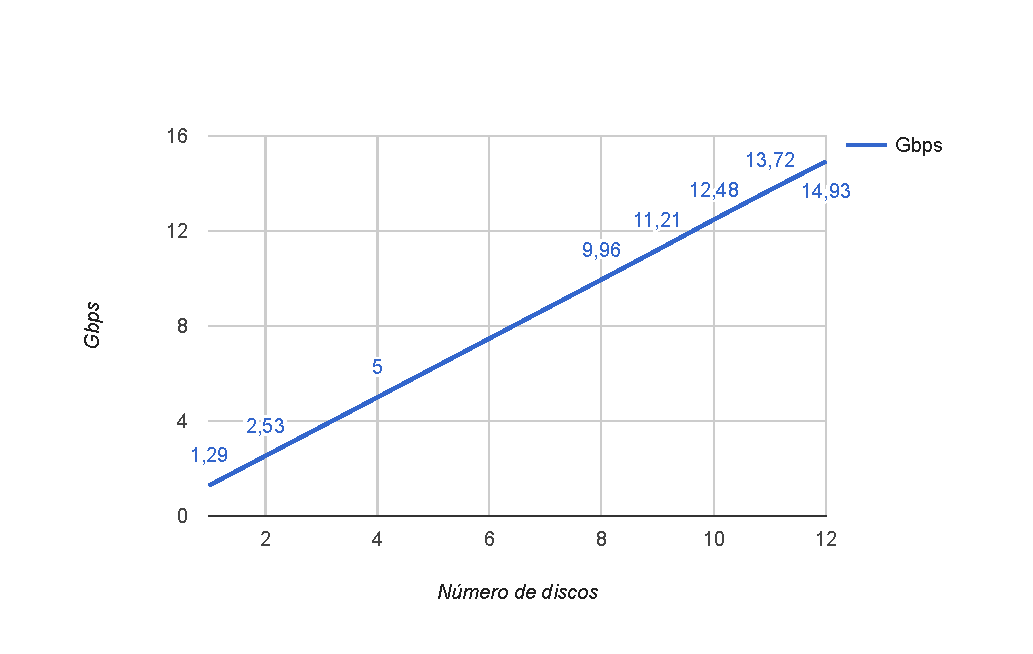
\includegraphics[scale=.7]{graph2}
\caption{Rendimiento de escritura en Raid 0 utilizando VirtIO}
\label{fig:vmfisica:graphdd2}
\end{figure}

\newpage
\subsection{Usando Passthrough\label{sec:pt}}

Dentro de los modelos de virtualización clásicos, nos encontramos con el modelo de \gls{passthough}. Este sistema de virtualización consiste en transferir todo el control sobre un determinado dispositivo a la máquina virtual. De esta forma, una \gls{vm}, es capaz de utilizar los driver nativos para susodicho dispositivo mitigando enormemente los efectos de la virtualización.

A pesar de que en términos de rendimiento la tecnología de \gls{passthough} se encuentra aventajada, esta forma de virtualización no permite que los recursos se compartan. Recordemos que una de las premisas de la virtualización es la compartición de recursos, ya que se asume que una única máquina virtual usualmente no explota al 100\% todos los recursos de los que dispone. En la figura~\ref{fig:vmpass} se muestra una arquitectura en la cual existen diversas máquinas virtuales. No obstante, aunque las aplicaciones dentro de una máquina virtual pueden compartir el harware, las aplicaciones de otras \glspl{vm} requieren sus propios dispositivos.

\begin{figure}[!htb]
\centering
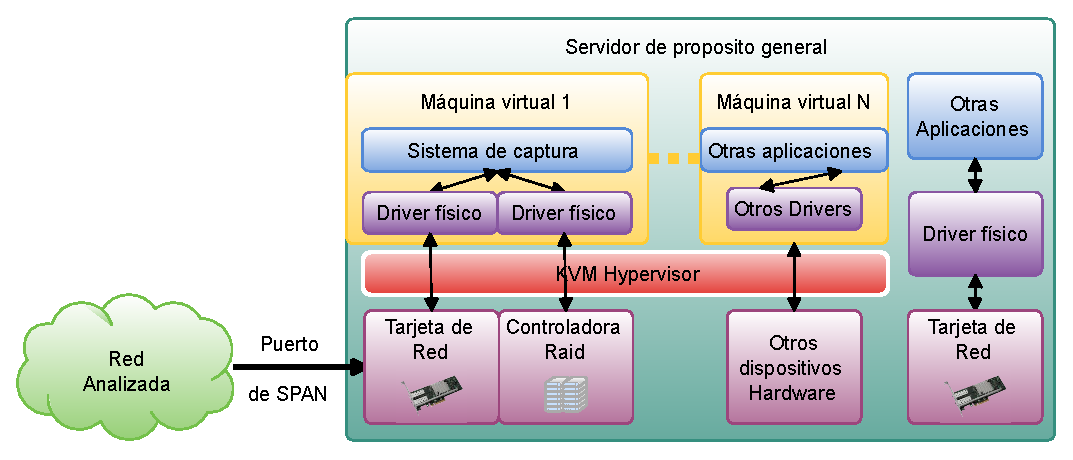
\includegraphics[scale=.6]{VMPass}
\caption{Arquitectura de captura en un escenario con Passthrough} 
\label{fig:vmpass}
\end{figure}

Bajo este paradigma de virtualización, se han vuelto a repetir las pruebas de escritura en el raid. Dado que la máquina virtual gestiona la controladora raid de la misma forma que lo haría una máquina real, el rendimiento se ve muy poco alterado con el rendimiento medido en un entorno real. Los resultados de estas pruebas pueden verse en la figura~\ref{fig:vmfisica:graphdd3}.

\begin{figure}[!htb]
\centering
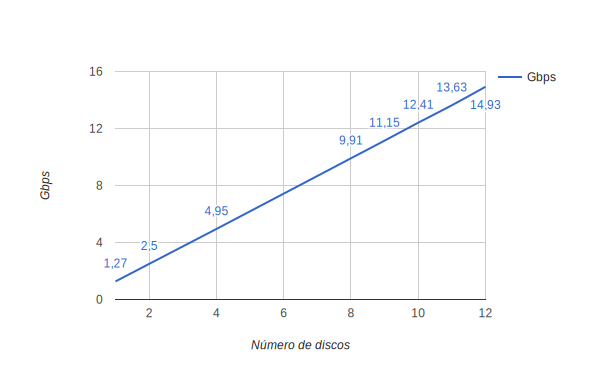
\includegraphics[scale=.7]{graph3}
\caption{Rendimiento de escritura en Raid 0 utilizando Passthrough}
\label{fig:vmfisica:graphdd3}
\end{figure}

Una de las ventajas que aportan las tarjetas de red de 10~\gls{gbps} de Intel es la representación de cada \gls{nic} como un dispositivo PCIe independiente. Esto permite que cada interfaz de la tarjeta de red pueda ser utilizada por una máquina diferente, ya sea esta física o virtual. Con el objetivo de observar como afecta dividir el tráfico entre un entorno físico y un entorno virtual, se han realizado pruebas en las siguientes 3 arquitecturas: 1 \gls{nic} en una única máquina virtual, 2 \glspl{nic} en una única máquina virtual y 2 \glspl{nic} (1+1) repartidas entre una máquina virtual y su sistema operativo anfitrión. Los resultados de la prueba de solo captura pueden verse en la taba~\ref{tab:vmpass:soloCap}.

\begin{table}[htb]
\centering
\begin{tabular}{|c|c|c|c|c|c|c|}
	\hline
		\multirow{3}{*}{\begin{tabular}[c]{c}{\bf Motor}\\ {\bf de captura}\end{tabular}} & \multicolumn{6}{c|}{{\bf \% de paquetes procesados}}\\
	\cline{2-7}
		 & \multicolumn{2}{c|}{{\bf 1 \gls{nic}}} & \multicolumn{2}{c|}{{\bf 2 \glspl{nic}}} & \multicolumn{2}{c|}{{\bf 1+1 \glspl{nic}}} \\
	\cline{2-7}
		 & {\bf 64 Bytes }   & {\bf CAIDA}  & {\bf 64 Bytes}   & {\bf CAIDA} & {\bf 64 Bytes}   & {\bf CAIDA}  \\ \hline
		ixgbe         & 1.9   & 62.7    & 2.5   & 41.8     & 6.2   & 83.7   \\ \hline
		PF\_RING      & 99.8  & 100     & 75.2  & 100      & 99.7  & 100    \\ \hline
		HPCAP         & 85.2  & 100     & 33.6  & 99.9     & 89.9  & 100    \\ \hline
		DPDK          & 100   & 100     & 100   & 100      & 100   & 100    \\ \hline
\end{tabular}
\caption{Porcentaje de paquetes capturados mediante Passthrough sin almacenamiento de paquetes.}
\label{tab:vmpass:soloCap}
\end{table}

En los resultados mostrados por la tabla anterior, se aprecia una pequeña degradación en el rendimiento cuando una única máquina virtual gestiona más de 1 \gls{nic}. Es probable que este efecto se deba a que cada una de las \glspl{vm} tiene un número de recursos limitado inferior al del sistema operativo anfitrión. Si los motores de captura requieren más recursos (ya sean \glspl{core} o memoria) y no disponen de ellos, inevitablemente el rendimiento se ve afectado.

\begin{table}[htb]
\centering
\begin{tabular}{|c|c|c|c|c|}
	\hline
		\multirow{3}{*}{\begin{tabular}[c]{c}{\bf Motor}\\ {\bf de captura}\end{tabular}} & \multicolumn{4}{c|}{{\bf \% de paquetes procesados}}\\
	\cline{2-5}
		 & \multicolumn{2}{c|}{{\bf Raid en Passthrough}} & \multicolumn{2}{c|}{{\bf Raid en VirtIO}} \\
	\cline{2-5}
		 & {\bf 64 Bytes }   & {\bf CAIDA}  & {\bf 64 Bytes}   & {\bf CAIDA}  \\ \hline
		HPCAP         & 82.2  & 100    & 82.8    & 100     \\ \hline
		DPDK          & 97.6  & 100    & 95.3    & 100  \\ \hline
\end{tabular}
\caption{Porcentaje de paquetes almacenados en un escenario con Passthrough.}
\label{tab:vmpass:CapAlmac}
\end{table}

Finalmente, en la tabla~\ref{tab:vmpass:CapAlmac}, se muestran los resultados de las pruebas de realizar almacenamiento y captura simultáneamente sobre una única máquina virtual. Esta tabla muestra a su vez el rendimiento de captura del sistema tanto cuando el raid se encuentra conectado mediante \gls{virtio}, como cuando se encuentra conectado mediante \gls{passthough}. Es interesante observar nuevamente el efecto de las filosofías \gls{onecopy} y \gls{zerocopy}. A pesar de que la escritura mediante \gls{virtio} mejora ligeramente el rendimiento del raid, las copias intermedias causan un breve aumento en la latencia y duración del pipeline de proceso. Mientras que el motor de captura \gls{dpdk} se ve afectado negativamente por el aumento de este retardo, el motor de captura \textit{HPCAP} tiene una mayor independencia y se ve beneficiado por el aumento de velocidad medio.


\subsection{Usando SR-IOV\label{sec:sriov}}

La tecnología \gls{sriov} ofrece multitud de ventajas frente a los otros métodos de virtualización, no sin por supuesto, traer nuevos inconvenientes. La mayor ventaja que ofrece \gls{sriov} es la compartición de recursos, al igual que lo es su mayor desventaja, pues se crea un cuello de botella. Cuando hablamos de \gls{sriov} en redes de comunicaciones, comúnmente estamos hablando de \gls{nfv}, es decir funciones virtuales de una determinada interfaz de red. Recordemos, que para que una tarjeta de red pueda crear diversas \glspl{nfv}, es necesario que la tarjeta física actúe a su vez como un switch entre las diferentes \glspl{nfv}. Esto aporta cierto valor añadido, pues mejora la comunicación interna entre las diferentes máquinas virtuales. Como contraparte, da un mayor trabajo a la tarjeta de red.

Dentro de este contexto, surge una nueva arquitectura de captura de tráfico. Dado que existen \glspl{nfv} en nuestro escenario, la aplicación de captura comparte las interfaces con otras aplicaciones de red (como puede ser un servidor web apache, una base de datos, o cualquier aplicación que utilice la red). Todas estas aplicaciones, tanto en máquinas máquinas virtuales, como en el propio anfitrión, utilizan un driver virtual para explotar un segmento de los recursos físicos de la tarjeta de red.
En la figura~\ref{fig:vmsriov} se presenta una arquitectura de captura en la que hay presentes diferentes elementos todos ellos conectados mediante \gls{sriov} y drivers virtuales. Nótese, que siguen existiendo elementos (la controladora Raid) que siguen siendo virtualizados con \gls{passthough} pues no disponen de \gls{sriov}.

\begin{figure}[!htb]
\centering
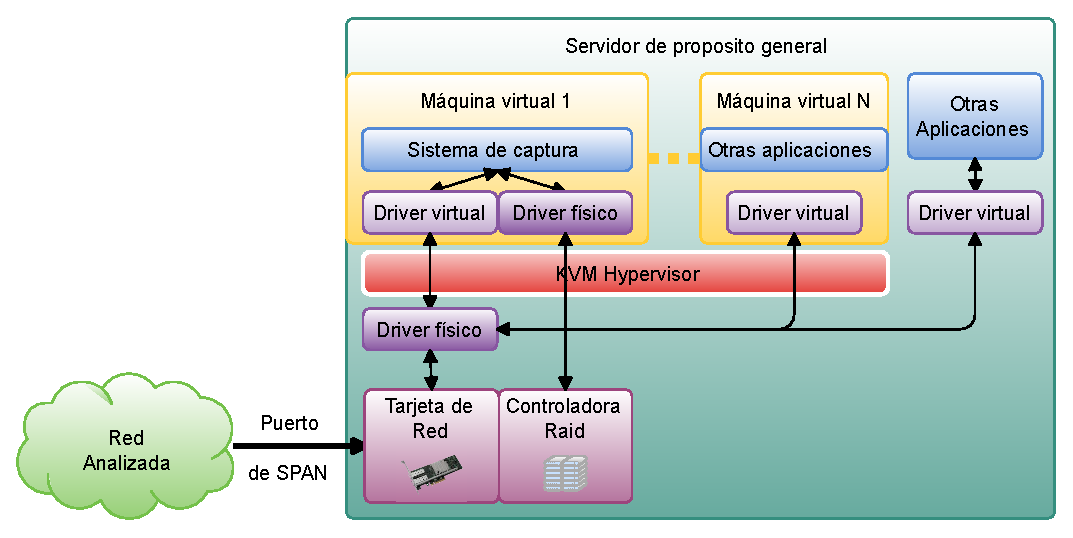
\includegraphics[scale=.7]{VMsriov}
\caption{Arquitectura de captura en un escenario con SRIOV y NFVs}
\label{fig:vmsriov} 
\end{figure}

%contar la diferencia de generación de NFV
\subsubsection{Comparativa de construcción de \glspl{nfv}}

Para que un dispositivo genere funciones virtuales, es necesaria la presencia de un driver en la máquina anfitriona que configure el dispositivo físico (número de \glspl{vf}, tamaños de las colas, reparto de interrupciones, etc). Para el caso de las tarjetas de Intel de 10~\gls{gbps}, el driver \gls{vanilla} ofrece esta funcionalidad de una manera muy cómoda. Este driver cumple con la filosofía de \gls{sriov} de delegar en la tarjeta todo el proceso de reparto de interrupciones y paquetes entre las diferentes \gls{nfv}.

No obstante, Intel ofrece una segunda forma de gestionar estas \glspl{nfv}. Los drivers de \gls{dpdk} permiten a su vez generar estas funciones virtuales, pero a diferencia del driver \textit{ixgbe}, es necesario ejecutar un programa sobre \gls{dpdk} para que estas \gls{nfv} reciban tráfico. El programa, conocido como \textit{testpmd}, ayuda activamente a la tarjeta liberándola en parte de la lógica que supone realizar de switch y la copia de paquetes entre la cola de recepción física y las colas asociadas a cada función virtual.
A su vez este programa permite configurar elementos a muy bajo nivel de la tarjeta, que en el driver \textit{ixgbe} supondría modificar el código del propio driver.

En la tabla~\ref{tab:vmsriov:sriov} se muestra una comparativa entre los diferentes métodos de generación de \gls{nfv}. Claramente, parece que el sistema de generación mediante \gls{dpdk} supera por mucho en rendimiento al driver \gls{vanilla}. Por otro lado, para que la aplicación \textit{testpmd} funcione a pleno rendimiento, es necesario reservarla un \gls{core} completo por cada función virtual, al igual que otro \gls{core} para ejecutar la interfaz. Esta limitación obliga a la larga a disponer de un gran número de cores que tan solo copian paquetes entre colas físicas y virtuales.

\begin{table}[htb]
\centering
\begin{tabular}{|c|c|c|}
	\hline
		\multirow{2}{*}{\begin{tabular}[c]{c}{\bf Motor}\\ {\bf de captura}\end{tabular}} & \multicolumn{2}{c|}{{\bf \% de paquetes procesados}}\\
	\cline{2-3}
		 & {\bf Gen. Ixgbe }   & {\bf Gen. \gls{dpdk}}    \\ \hline
		ixgbevf         & >0.1  & 1     \\ \hline
		HPCAPvf         & 36.2  & 82.7     \\ \hline
		DPDK            & 37.6  & 100    \\ \hline
\end{tabular}
\caption{Porcentaje de paquetes capturados en función del método de generación de NFV. El tráfico utilizado estaba formado por paquetes de tamaño mínimo (64Bytes).}
\label{tab:vmsriov:sriov}
\end{table}


\subsubsection{Pruebas de recepción con \glspl{nfv}}

De cara a realizar pruebas con \glspl{nfv}, es necesario mencionar algunos detalles implementativos. Cada \gls{nfv}, a diferencia de su hermana física, tiene una única cola de recepción y transmisión. Por temas de diseño, las \glspl{nfv} tampoco cuentan con contadores de paquetes perdidos, o erróneos, por lo que obtener estos datos es necesario inferirlos de las estadísticas que ofrecen las funciones físicas. Por este motivo, no se han podido medir con exactitud las pérdidas en los diferentes escenarios con \gls{nfv}, no obstante, se han obtenido datos bastante aproximados.

Como se ha mencionado anteriormente, la tarjeta física, es la encargada en última instancia de gestionar hacia que \gls{nfv} se envía cada uno de los paquetes recibidos. Para determinarlo, cada \gls{nfv} posee su propia dirección MAC virtual. Con el objetivo de probar la escalabilidad en función de máquinas virtuales y \glspl{nfv} por \gls{nic} física, se han utilizado 3 máquinas virtuales con dos 2 \glspl{core} virtuales cada una.
Cada \gls{vm} cuenta con una \gls{nfv} con MAC única. Para medir el rendimiento, estas máquinas virtuales ejecutan en paralelo la versión de solo captura desarrollada en \gls{dpdk}. Para realizar las pruebas se han creado 3 trazas de tráfico sinténtico. La primera traza contiene paquetes de tamaño 64 Bytes, todos ellos con una única dirección MAC. La segunda traza, contiene 2 direcciones MAC en una proporcion del 50\% cada una. La tercera traza, contiene 3 direcciones MAC, en una proporcion del 33.3\% cada una.

Los resultados obtenidos de las pruebas figura en la tabla~\ref{tab:vmsriov:rnfv}. En esta tabla, se pueden observar ligeras pérdidas pues no se llegan a alcanzar los 10~\gls{gbps}. No obstante, el rendimiento parece escalar y no se ve aparentemente afecto por el número de \glspl{nfv} que hay en el sistema o el número de máquinas virtuales en ejecución.

\begin{table}[htb]
\centering
\begin{tabular}{|c|c|c|}
	\hline
		\multirow{2}{*}{\begin{tabular}[c]{c}{\bf Número de}\\ {\bf MACs emitidas}\end{tabular}} & \multicolumn{2}{c|}{{\bf \% de paquetes procesados}}\\
	\cline{2-3}
		 & {\bf Por cada \gls{vm} }   & {\bf En total}    \\ \hline
		1         & 99.5  & 99.5     \\ \hline
		2         & 49.7  & 99.4     \\ \hline
		3         & 33.2  & 99.5     \\ \hline
\end{tabular}
\caption{Porcentaje de paquetes capturados en función del número de VMs y de direcciones MAC destino}
\label{tab:vmsriov:rnfv}
\end{table}

\subsubsection{\glspl{nfv} con captura promíscua}

No obstante, el método nativo de funcionamiento de las \gls{nfv}, no nos sirve para poder construir una sonda de tráfico virtual, pues en un principio solo seríamos capaces de capturar el tráfico destinado a nuestra función virtual. Si el objetivo de nuestro sistema es ofrecer un servicio por una determinada interfaz y a la vez capturar por esta, podemos recurrir a la bandera \gls{mpe}~\cite{825992010}. Esta bandera puede ser configurada a través del programa \textit{testpmd}, e indica a la tarjeta que reenvíe todos aquellos paquetes sin destino conocido a una determinada \gls{nfv}. Nótese, que esta aproximación no nos reenvía aquellos paquetes destinados a una dirección MAC asociada a otra \gls{nfv} de nuestro sistema. No obstante, esta aproximación es sencilla y permite a la tarjeta funcionar a alta velocidad, además de ser completamente válida si mantenemos la arquitectura del típico puerto de SPAN.

En la tabla~\ref{tab:vmvirtio:soloCapA} se muestran los resultados de solo captura. En este escenario, se pretende probar el rendimiento que ofrecen las \glspl{nfv} bajo condiciones habituales. Para ello, se realizan 3 pruebas simples: Una única \gls{vm} conectada a una \gls{nfv}, una única \gls{vm} conectada a dos \gls{nfv} (cada una correspondiente a una \gls{nic} diferente) y finalmente, 2 \glspl{vm} conectadas a 2 \gls{nfv} generadas a partir de la misma \gls{nic}.
%
Los resultados de la tabla son en parte similares a otras pruebas ya realizadas, aunque caben destacar algunos resultados. Para el caso de \textit{HPCAPfv}, al gestionar 2 \glspl{nfv} en una máquina virtual con pocos recursos, se ve saturado rápidamente y el rendimiento cae por falta de \glspl{core}. En el caso de utilizar dos máquinas virtuales en paralelo compartiendo \gls{nic}, se observa que tanto en el motor \gls{dpdk} como en el motor de captura\textit{HPCAPvf}, tienen resultados similares. Esta última prueba de doble \gls{nfv} y doble \gls{vm}, se realizó mediante una traza de paquete mínimo con la MAC destino a broadcast, de forma que todos las \glspl{nfv} recibieran todos y cada uno de los paquetes. Si tenemos esto en cuenta, aunque el tráfico que llega por la interfaz se recibe a 10~\gls{gbps}, la tarjeta debe enviar datos a las diferentes \glspl{nfv} a 20~\gls{gbps}. Con esto en mente, el 51\% o el 44.1\% de 20~\gls{gbps}, se asemeja mucho a valores obtenidos anteriormente.

\begin{table}[htb]
\centering
\begin{tabular}{|c|c|c|c|c|c|c|}
	\hline
		\multirow{3}{*}{\begin{tabular}[c]{c}{\bf Motor}\\ {\bf de captura}\end{tabular}} & \multicolumn{6}{c|}{{\bf \% de paquetes procesados}}\\
	\cline{2-7}
		 & \multicolumn{2}{c|}{{\bf 1 \gls{nfv}}} & \multicolumn{2}{c|}{{\bf 2 \glspl{nfv}}} & \multicolumn{2}{c|}{{\bf (1+1) 2\glspl{nfv}/2\glspl{vm}}} \\
	\cline{2-7}
		 & {\bf 64 Bytes }   & {\bf CAIDA}  & {\bf 64 Bytes}   & {\bf CAIDA} & {\bf 64 Bytes}   & {\bf CAIDA}  \\ \hline
		ixgbePvf      & 1     & 34.2    & 1     & 42.4     & 0.9   & 14.8    \\ \hline
		HPCAPvf       & 82.7  & 100     & 13.0  & 100      & 44.1  & 82.7    \\ \hline
		DPDK          & 100   & 100     & 100   & 100      & 50.8  & 83.0    \\ \hline
\end{tabular}
\caption{Porcentaje de paquetes capturados y no almacenados en un escenario con SRIOV y flag MPE.}
\label{tab:vmvirtio:soloCapA}
\end{table}

%%%%
En la tabla~\ref{tab:vmvirtio:CapAlmac1} se muestran los resultados de captura y almacenamiento cuando solo hay una única \gls{nfv} y una única \gls{vm} en ejecución. Es interesante apreciar como la sobrecarga de la virtualización con \gls{virtio} y \gls{nfv} incrementa lo suficiente la latencia del pipeline de captura de la herramienta de \gls{dpdk} como para hacerla perder una enorme cantidad de paquetes.

\begin{table}[htb]
\centering
\begin{tabular}{|c|c|c|c|c|}
	\hline
		\multirow{3}{*}{\begin{tabular}[c]{c}{\bf Motor}\\ {\bf de captura}\end{tabular}} & \multicolumn{4}{c|}{{\bf \% de paquetes procesados}}\\
	\cline{2-5}
		 & \multicolumn{2}{c|}{{\bf Raid en Passthrough}} & \multicolumn{2}{c|}{{\bf Raid en VirtIO}} \\
	\cline{2-5}
		 & {\bf 64 Bytes }   & {\bf CAIDA}  & {\bf 64 Bytes}   & {\bf CAIDA}  \\ \hline
		HPCAPvf       & 82.6  & 100    & 82.3    & 100     \\ \hline
		DPDK          & 94.2  & 100    & 68.2    & 100  \\ \hline
\end{tabular}
\caption{Porcentaje de paquetes almacenados en un escenario con SRIOV y flag MPE.}
\label{tab:vmvirtio:CapAlmac1}
\end{table}

\subsubsection{\glspl{nfv} con captura global}

En las secciones anteriores de \glspl{nfv}, se ha hablado acerca de como funciona el reparto de paquetes entre las diferentes funciones y de como es posible capturar tráfico que no va destinado a ninguna función virtual. No obstante, uno de los objetivos de este trabajo es evaluar el proceso de monitorización en redes virtuales. Para lograrlo, el datasheet de las tarjetas de Intel~\cite{825992010} nos proporciona información acerca del concepto de \textit{Port Mirroring}. A través de una serie de registros, es posible indicar a la tarjeta de red, que copie todos los paquetes que entren o salgan de una cola a otra cola. Dado que cada \gls{nfv}, tiene asociada una única cola, es posible forzar la copia del contenido de una \gls{nfv} a otra \gls{nfv}. Toda esta configuración de \textit{mirroring} puede ser configurada a través de la aplicación \textit{testpmd}.

La idea principal para realizar esta prueba consiste en utilizar las 3 máquinas virtuales mencionadas al inicio de esta subsección como consumidoras de tráfico, mientras que una cuarta máquina virtual, con la configuración estándar utilizada hasta ahora(y descrita en la sección~\ref{sec:sw}), monitorice el tráfico entre dichas \glspl{vm}.
Dado que el equipo de pruebas tiene arquitectura \gls{numa} y los recursos de las 4 \glspl{vm} exceden los recursos de un procesador, es necesario distribuir las diferentes \glspl{vm} entre los procesadores. Dado que la localización de las \gls{vm} puede afectar al rendimiento, se ha decidido agrupar las 3 \glspl{vm} consumidoras en un mismo procesador, pues comparten funcionalidad similar, y la \gls{vm} de monitorización en otro procesador. 

En la tabla~\ref{tab:vmvirtio:CapAlmac2} se muestra un breve resumen de las pruebas realizadas. Por un lado, los resultados muestran una tasa acotada de \gls{gbps} que pueden ser capturados mediante este método. Dado que el \textit{Port Mirroring} consiste en duplicar todos y cada uno de los paquetes, el hecho de que el rendimiento decrezca es razonable, pues en definitiva se están recibiendo al menos el doble \gls{gbps}.
Un dato curioso, son los resultados de rendimiento. Si recordamos la arquitectura de la sonda de prueba, el tarjeta de red se encuentra conectada en el nodo \gls{numa}. Dado que este nodo es el más cercano a la tarjeta, parece razonable ejecutar la \gls{vm} en este nodo. No obstante, cuando la \gls{vm} es capaz de capturar mucho más tráfico cuando se encuentra en el nodo \gls{numa} 1.
Este efecto ha de tenerse en cuenta, pues el \textit{Port Mirroring}, no redirige los paquetes a la \gls{vm} de captura, salvo que dicho paquete ya haya sido atendido por la \gls{vm} adecuada. Por ello, situar las máquinas consumidoras en el nodo más cercano a la tarjeta favorece la cantidad de paquetes capturados mediante la técnica del \textit{Port Mirroring}.

\begin{table}[!htb]
\centering
\begin{tabular}{|c|c|c|c|}
	\hline
	\multirow{2}{*}{\begin{tabular}[b]{c}{\bf Motor}\\ {\bf de captura}\end{tabular}} & \multirow{2}{*}{\begin{tabular}[b]{c}{\bf Nodo Numa}\\ {\bf de captura}\end{tabular}} & \multicolumn{2}{c|}{{\bf \% de paquetes procesados}}\\
	\cline{3-4}
	& &  {\bf 64 Bytes } & {\bf CAIDA} \\
	\hline
			\multirow{2}{*}{HPCAPvf} & 0  &  30.7   &  48.0  \\
		\cline{2-4} 
			& 1  &   47.4  &  76.7  \\
	\hline
			\multirow{2}{*}{DPDK} & 0  &  22.8   & 38.4   \\
		\cline{2-4} 
			& 1  &   50.4  &  76.8  \\
	\hline
\end{tabular}
	\caption{Porcentaje de paquetes almacenados en un escenario con SRIOV y Port Mirroring. Captura del tráfico interno de una red virtual formada por 3 VMs. El raid de almacenamiento se encuentra configurado con VirtIO}
	\label{tab:vmvirtio:CapAlmac2}
\end{table}


\subsubsection{Sistema distribuido de monitorización}

Aunque las pruebas de rendimiento mostradas en la tabla~\ref{tab:vmvirtio:CapAlmac2} parece que no son excepcionales, debemos recordar que encontrar un único servidor capaz de saturar un enlace a 10~\gls{gbps} resulta complicado incluso si sus servicios no sufren de ningún tipo de virtualización. Por otro lado, los servicios de virtualización se nutren de utilizar grandes cantidades de máquinas virtuales relativamente pequeñas.

A partir de este concepto, nace la idea de un sistema de monitorización y captura de tráfico distribuido. El coste de añadir una pequeña máquina virtual encargada de recolectar el tráfico de las demás \glspl{vm} con las que comparte anfitrión, es muy bajo. Dado que todas estas máquinas virtuales tienen una vía de comunicación entre sí, basta con añadir una nueva \gls{vm} que de forma transparente sea capaz de realizar un análisis con los datos capturados de cada una de las mini-sondas de captura virtuales. No obstante, construir y experimentar con este tipo de sistema distribuido queda fuera del alcance de este trabajo, aunque será considerada su realización como trabajo futuro






%
% Resultados
%
%\chapter{Resumen de resultados y comparativas\label{sec:resultados}}

A lo largo del capítulo~\ref{sec:desarrollo}, se han explicado las diferentes pruebas realizadas de los elementos que conforman los sistemas de captura y almacenamiento tanto en entornos físicos como virtuales.


\begin{table}[htb]
	\centering
	%\renewcommand{\arraystretch}{1.2}
	\begin{tabular}{|c|c|c|c|}
		\hline
		\multirow{3}{*}{\begin{tabular}[c]{c}{\bf Número}\\ {\bf de discos}\end{tabular}} & \multirow{3}{*}{{\bf Modo}} & \multicolumn{2}{c|}{{\bf Rendimiento (Gbps)}} \\
		\cline{3-4} 
		& & {\bf Media} & \begin{tabular}[c]{c}{\bf Intervalo de confianza}\\ ($\alpha$=0.01)\end{tabular} \\
		\hline
		\multirow{3}{*}{1} & Físico   & 1.27    & (1.27, 1.28)     \\
		\cline{2-4} 
		& \gls{virtio}         & 1.29    & (1.25, 1.34) \\
		\cline{2-4} 
		& \gls{passthough}          & 1.27    & (1.27, 1.28)   \\
		\hline
		\multirow{3}{*}{8} & Físico     & 9.93    & (9.89, 9.96) \\
		\cline{2-4} 
		& \gls{virtio}          & 9.96    & (9.79, 10.13) \\
		\cline{2-4} 
		& \gls{passthough}            & 9.91    & (9.85, 9.96) \\
		\hline
		\multirow{3}{*}{9} & Físico    & 11.16   & (11.09, 11.23) \\
		\cline{2-4} 
		& \gls{virtio}         & 11.21   & (11.03, 11.39) \\
		\cline{2-4} 
		& \gls{passthough}           &  11.15 & (11.09, 11.21) \\
		\hline
	\end{tabular}
	\caption{Tasa de escritura en Raid 0, en función del modo de funcionamiento (físico o con virtualización) y el número de discos}
	\label{tab:raidperf}
\end{table}


\begin{table}[htb]
\centering
\begin{minipage}[c]{\textwidth}
\resizebox{\textwidth}{!}{
\begin{tabular}{|c|c|c|c|c|c|c|}
	\hline
	\multicolumn{2}{|c|}{  \multirow{2}{*}{{\bf I/O configuration}  }} & \multirow{3}{*}{\begin{tabular}[b]{c}{\bf Capture}\\ {\bf engine}\end{tabular}} & \multicolumn{4}{c|}{{\bf \% of packets processed}}   \\
	\cline{4-7}
	\multicolumn{2}{|c|}{}  &  & \multicolumn{2}{c|}{  {\bf 64-byte packets}  } & \multicolumn{2}{c|}{  {\bf CAIDA trace}  }  \\
	\cline{1-2} \cline{4-7} 
	{\bf Network} & {\bf Storage} &  &  \begin{tabular}[c]{c}{\bf Capture}\\{\bf only}\end{tabular} &  \begin{tabular}[c]{c}{\bf Capture}\\{\bf and storage}\end{tabular} & \begin{tabular}[c]{c}{\bf Capture}\\{\bf only}\end{tabular} &\begin{tabular}[c]{c}{\bf Capture}\\{\bf and storage}\end{tabular} \\
	\hline
		\multicolumn{2}{|c|}{\multirow{2}{*}{Bare-metal}} & DPDK & 100.0 & 95.8 & 100.0 & 100.0\\
		\cline{3-7} 
		\multicolumn{2}{|c|}{} & HPCAP & 97.9 & 95.7 & 100.0 & 100.0 \\
	\hline
			\multirow{4}{*}{PT} & \multirow{2}{*}{PT}     & DPDK     & 100.0    &    97.6    & 100.0    &  100.0 \\
			\cline{3-7} 
			& & HPCAP        & 85.2      &    82.3    & 100.0 &  100.0  \\
		\cline{2-7} 
		 & \multirow{2}{*}{VirtIO} & DPDK   & 100.0    &  95.3  & 100.0  & 100.0  \\
		 \cline{3-7}
		 &     & HPCAP      & 85.2  &  82.8 & 100.0    &  100.0 \\
	\hline
			\multirow{4}{*}{VF} &  \multirow{2}{*}{PT}    & DPDK    & 100.0   &   94.2   & 100.0   & 100.0  \\
			\cline{3-7} 
			&   & HPCAPvf     & 82.7    &  82.6  & 100.0   &  100.0 \\
		\cline{2-7} 
			 & \multirow{2}{*}{VirtIO} & DPDK   & 100.0   & 68.0   & 100.0  & 100.0   \\
			 \cline{3-7}
			 &     & HPCAPvf  & 82.7  & 82.3  & 100.0 & 100.0 \\
	\hline
\end{tabular}
}
\end{minipage}
	\caption{Percentage of packets processed for diverse virtual I/O configuration in a network probe for packet capture only and packet capture and storage.}
	\label{tab:virtcapwr}
\end{table}

%
% Conclusiones
%
\chapter{Conclusiones\label{chap:conclusiones}}

TODO: Conclusiones sobre el trabajo realizado 

%
% Página en blanco
%
\cleardoublepage

%
% Bibliografía
%
% Rerefencias
\bibliographystyle{IEEEtran}
\bibliography{src/bibliografia}
\addcontentsline{toc}{chapter}{Bibliografía}

% No expandir elementos para llenar toda la página
\raggedbottom

%
% Apéndices
%
\appendix
\cleardoublepage
\addappheadtotoc
\appendixpage

%
% TODO: Apéndices del TFG
%
\chapter{Towards high-performance network processing in virtualized environments\label{sec:HPCC}}

El artículo publicado se titula `` Towards high-performance network processing in virtualized environments '' y ha sido enviado al congreso HPCC, el cual está catalogado como \textbf{\href{http://103.1.187.206/core/?search=hpcc&by=all&source=CORE2014&sort=atitle&page=1}{CORE B}}. A continuación, se muestra la carta de aceptación, las revisiones y finalmente el artículo en sí.

\section{Email de aceptación}

\begin{verbatim}
 Fecha:	 6 de junio de 2015, 21:29:31 CEST
 De:	 HPCC 2015 <hpcc2015@easychair.org>
 Para:	 Víctor Moreno <victor.moreno@uam.es
 Asunto: HPCC 2015 notification for paper 51
\end{verbatim}
\begin{verbatim}
Dear Víctor,

Thank you for your contribution to IEEE HPCC 2015.

Congratulations! Your paper #51, titled as "Towards high-performance network
processing in virtualized environments", has been officially accepted as a
full paper for publication and presentation in IEEE HPCC 2015.

Please check reviewers' comments, and prepare your final version based on IEEE
conference proceeding format. The size of your final paper should be up to 6
pages complimentary, or 12 pages with the over length charge.

The completed reviews are attached below.

In order to publish your article, please prepare your final camera ready version
according to the requirements on IEEE HPCC website. 

We will send you the detailed instruction about your final submission in another
mail later.

Please prepare your trip (visa, air ticket, hotel) in advance. See you at
New York City.

Best,
PC Chairs of IEEE HPCC 2015
\end{verbatim}

\section{Revisiones}
\subsection{Revisor 1}
\begin{verbatim}
OVERALL EVALUATION: 0 (borderline paper)
REVIEWER'S CONFIDENCE: 4 (high)

----------- REVIEW -----------
This paper presents a study on some of the existing network processing techniques
in different configurations.  By comparing the package capturing capabilities and
performance, the authors claim that they provide the audience a series of guidelines
for network application deployment with low cost, high performance, space efficiency,
and low power consumption.

My major concern about the paper is its contribution. A large body of the paper is
devoted to presenting a preliminary investigation of several well known technologies
(PF_RING, Intel DPDK, HPCAP, etc.), omiting the detailed introduction to author's
own framework HPCAPvf.  The authors present their experimental results for various
configurations and techniques. However, I feel there is a lack of the experimental
details and methodology. To make their results more convincing, the authors should
include a methodology section dedicated to elaborate their experimental approach.
Too much space is taken to introduce the results, system structures and tradeoffs
for basic, well know concepts such as huge pages, package handling in virtualized
network, etc. Figure 4 and 5 take too much space.  The author should use more space
to introduce the details and techniques specific to this work.   Regarding the
presented results, why the authors use percentage of captured packages as a 
"perf!ormance" indicator of the compared techniques? I think this metric should be
used to indicate the accuracy, not the performance.

The paper is not well written. There are many typos and mistakes. Just to name a few:
In the sentence "traditional end-user network applications retrieves packets
individually by means of system calls, which in Linux systems involves at least two
context switches.", retrieves should be retrieve, involves should be involve.  This
sentence is long and reads awkward: "Those tests were made using the same hardware as
previously mentioned and using KVM for creating and managing the VMs, and accordingly
to the bare-metal scenario, the table depicts each capture engine’s performance for
the worst case scenario and in an average scenario.", and accordingly should be
according.  There are many other places that the author should do a proofreading.
\end{verbatim}

\subsection{Revisor 2}
\begin{verbatim}
OVERALL EVALUATION: 2 (accept)
REVIEWER'S CONFIDENCE: 2 (low)

----------- REVIEW -----------
This paper evaluates the performance of several well-known high-performance capture
engines on virtual machines. In addition, the paper presents an open-source version
of the HPCAP for virtual environments. The experimental results presented in this
paper are valuable for network operators that want to employ network virtual
functions.

The paper is well written and easy to understand even for a non-expert in this field.
The experimental results are based on a realistic benchmark and show insightful results.
\end{verbatim}

\section{Artículo}
Puede verse el artículo en la siguiente página.

\includepdf[pages={1,2,3,4,5,6,7,8}]{graphics/virtualHPCC.pdf}

% Fin del documento
\end{document}
